\documentclass[Royal,sageh,times]{sagej}
% Afour
\usepackage{moreverb,url}

\usepackage[colorlinks,bookmarksopen,bookmarksnumbered,citecolor=red,urlcolor=red]{hyperref}

\usepackage{chngpage}

\newcommand\BibTeX{{\rmfamily B\kern-.05em \textsc{i\kern-.025em b}\kern-.08em
T\kern-.1667em\lower.7ex\hbox{E}\kern-.125emX}}

\def\volumeyear{2017}


\usepackage[utf8]{inputenc}
\usepackage[T1]{fontenc}

%%%%%
% variable to include comments or not in the compilation ; set to 1 to include
%\def \draft {1}
\def \draft {0}



\usepackage{xparse}
\usepackage{ifthen}

\DeclareDocumentCommand{\comment}{o m o o o o}
{\ifthenelse{\draft=1}{
  \IfValueT{#1}{
      \textcolor{red}{\textbf{C (#1) : }#2}
      \IfValueT{#3}{\textcolor{blue}{\textbf{A1 : }#3}}
      \IfValueT{#4}{\textcolor{ForestGreen}{\textbf{A2 : }#4}}
      \IfValueT{#5}{\textcolor{red!50!blue}{\textbf{A3 : }#5}}
      \IfValueT{#6}{\textcolor{Aquamarine}{\textbf{A4 : }#6}}
    }
    \IfNoValueT{#1}{
      \textcolor{red}{\textbf{C : }#2}
      \IfValueT{#3}{\textcolor{blue}{\textbf{A1 : }#3}}
      \IfValueT{#4}{\textcolor{ForestGreen}{\textbf{A2 : }#4}}
      \IfValueT{#5}{\textcolor{red!50!blue}{\textbf{A3 : }#5}}
      \IfValueT{#6}{\textcolor{Aquamarine}{\textbf{A4 : }#6}}
    }
 }{}
}




% todo
%\newcommand{\todo}[1]{
%\ifthenelse{\draft=1}{\textcolor{red!50!blue}{\textbf{TODO : \textit{#1}}}}{}
%}
\DeclareDocumentCommand{\todo}{o m}{
  \ifthenelse{\draft=1}{
    \IfValueT{#1}{\textcolor{red!50!blue}{\textbf{TODO (#1) : \textit{#2}}}}
    \IfNoValueT{#1}{\textcolor{red!50!blue}{\textbf{TODO : \textit{#2}}}}
  }{}
}

%\date{}
%\renewcommand\abstractname{\fontsize{14pt}{0}\textbf{Abstract}\selectfont}

%\usepackage[left=25mm, right=25mm, top=25mm, bottom=25mm, includehead=false, includefoot=false]{geometry}

%\usepackage{graphicx}
%\usepackage{url}
%\usepackage[round,semicolon]{natbib}  % Citation styles https://www.sharelatex.com/learn/Natbib_citation_styles
%\bibliographystyle{humannat}
%\renewcommand{\bibsection}{}
%\renewcommand{\bibhang}{\setlength{-1px}}


%\usepackage{authblk} % For author lists
%\renewcommand\Authfont{\fontsize{11}{1}\selectfont}
%\renewcommand\Affilfont{\fontsize{9}{1}\selectfont}

%\renewcommand*\footnoterule{}

\usepackage[table]{xcolor}
\usepackage[parfill]{parskip} % Line between paragraphs
\usepackage{amsmath}
%\pagenumbering{arabic} 

%\usepackage{sectsty}
%\allsectionsfont{\sffamily}

%\usepackage[pdftex]{hyperref} 
%\hypersetup{pdfborder={0 0 0} }


\usepackage[flushleft]{threeparttable}



%%%%%%%%%%%%%%%%%%%%%%%%%
%% -- from ecrc template
%%%%%%%%%%%%%%%%%%%%%%%%%


%% set the volume if you know. Otherwise `00'
\volume{00}

%% set the starting page if not 1
\firstpage{1}



\jid{}


\biboptions{authoryear}




\usepackage{soul}
\soulregister\cite7
\soulregister\citep7
\soulregister\ref7

%\usepackage[final]{changes}
\usepackage{changes}


\setaddedmarkup{\textcolor{black}{\hl{#1}}}
\setdeletedmarkup{\textcolor{red}{\sout{#1}}}

% add line number
\usepackage{lineno}
\linenumbers








\begin{document}

% **************  TITLE AND AUTHOR INFORMATION **************


%\runninghead{Raimbault \& al.}
\runninghead{}

\title{Initial spatial conditions in simulation models: the missing leg of sensitivity analyses?}

%\author{Juste Raimbault\affilnum{1,2}, 
%Cl{\' e}mentine Cottineau\affilnum{3,4},
%Marion Le Texier\affilnum{5}, 
%Florent Le N{\' e}chet\affilnum{2}, 
%Romain Reuillon\affilnum{1,6}
%}
\author{}

%\affiliation{\affilnum{1}UMR 8504 G{\'e}ographie-cit{\'e}s, Paris, France\\
%\affilnum{2}Laboratoire Ville Mobilit{\'e} Transport, Universit{\'e} Paris-Est, France\\
%\affilnum{3}Centre for Advanced Spatial Analysis, University College London, UK\\
%\affilnum{4}CNRS, UMR 8097 Centre Maurice Halbwachs, Paris, France\\
%\affilnum{5}UMR 6266 IDEES, Universit{\'e} de Rouen Normandie, France\\
%\affilnum{6}Institut des Syst{\`e}mes Complexes Paris Ile-de-France, France}


%\corrauth{Juste Raimbault, UMR CNRS 8504 G{\'e}ographie-cit{\'e}s
%13 rue du Four,
%75006 Paris, France.
%\email{juste.raimbault@polytechnique.edu}}
%\corrauth{}



% authors bio
% Juste Raimbault is a PhD student at Université Paris 7, UMR CNRS 8504 Géographie-cités and UMR-T 9403 IFSTTAR LVMT, under the supervision of Arnaud Banos and Florent Le Néchet. He holds an engineer degree from Ecole Polytechnique and Ecole des Ponts et Chaussées, and a Master in Complex Systems Science from Ecole Polytechnique. His research focuses on complexity approaches to the relations between networks and territories.

% Dr. Clémentine Cottineau is a research associate at the Centre for Advanced Spatial Analysis of University College London. She studied geography and economics at University Paris 1 Panthéon-Sorbonne and holds a PhD in geography from this university. Her thesis aimed at modelling urbanisation in the post-Soviet space with modular agent-based models. Since 2014, she has been working at the Centre for Advanced Spatial Analysis on urban economics and parametric scaling in the context of European systems of cities, using tools from complexity science to investigate inequality in cities and economic disparities between cities.


% Cover Letter

% Dear editors,

%My coauthors and I are pleased to submit an original research article entitled ``Initial spatial conditions in simulation models: the missing leg of sensitivity analyses?'' for consideration for publication in Environment and Planning B. 

%This article deals with the central yet poorly explored issue of the sensitivity of geosimulation models to their spatial context (i.e. the spatial configuration of agents and their environment), and more precisely their spatial initial conditions. We think the subject in general and the novelty of the paper in particular will meet the interest of the readers of EPB, a journal dealing with urban modelling and city science.

%Despite some preliminary results being presented as at ECTQG 2015, Bari, and at Geocomputation Conference 2017, Leeds, we confirm that neither the manuscript nor any parts of its content are currently under consideration or published in another journal. We did not have any previous interaction with EPB regarding this manuscript. We have no conflicts of interest to disclose. We do not have any opposed reviewer.

% Yours faithfully,
% Juste Raimbault and co-authors.



% **************  ABSTRACT  **************

\begin{abstract}
%\noindent
%\setlength{\parindent}{0pt}
Although simulation models of geographical systems in general and agent-based models in particular represent a fantastic opportunity to explore socio-spatial behaviours and to test a variety of scenarios for public policy, the validity of generative models is uncertain until their results are proven robust and representative of 'real-world' conditions. Sensitivity analysis usually includes the analysis of the effect of stochasticity on the variability of results, as well as the effects of small parameter changes. However, initial spatial conditions are usually taken for granted in geographical models, thus leaving completely unexplored the effect of spatial arrangements on the interactions of agents and of that of agents with their environment. In this paper, we present a method to assess the effect of initial spatial conditions on simulation models, using a systematic generator controlled by meta-parameters in order to create the density grids with which spatial simulation models are initialised. We show, with the example of two classical agent-based models (Schelling's models of segregation and Sugarscape's model of resource harvesting) and a straightforward open-source work-flow using high performance computing, that the effect of space is significant in the two types of simulation. Furthermore, this effect is sometimes larger than the effect of parameters' value change. 
\end{abstract}

\keywords{Space, Initial conditions, Sensitivity, ABM, Validation}

\maketitle


% **************  MAIN BODY OF THE PAPER **************
%\newpage

%%%%%%%%%%%%%%%%%%%%%%
\section{Introduction}
%%%%%%%%%%%%%%%%%%%%%%

Simulation within computer models has been recognised and increasingly used by geographers as an efficient tool to explore geographical processes, hypotheses and predictive scenarios within virtual laboratories \citep{batty1971modelling, batty2007model, carley1999generating, Quesneletal2009}. %\comment{+ Seb \& James Doran in the 1970s??}
 Simulation also appears as a way to overcome the difficult analytic resolution of many spatial models which were developed in the past, as well as to explore the possible (alternative) trajectories of social and ecological systems in space and time. The specificity of geographical models compared to other social sciences' models is that space and spatial interactions are given a prime role, as geographers are driven by an explicit interest in studying the way space influences the outcomes of the model. Indeed, they usually seek to understand and model the role of space in social interactions and environmental processes, in a city for example. We think simulation can become a very good tool to achieve this, provided that models do include relevant spatial descriptions and behavioural rules which take space into account, and provided that the model evaluation includes a sensitivity analysis of output variations to the way space is modelled. Unfortunately, the first condition is not always met, and the second is seldom even mentioned. This paper aims to fill a methodological and conceptual gap, which is a systematic testing of the sensitivity of a model's outcomes to its initial spatial conditions. To demonstrate the genericity of our approach, we develop two applications with classic simulation models commonly used as case studies for comparing and aligning simulation models \citep{Axtelletal1996, wilensky2007making}: \citet{schelling1971dynamic}'s model of segregation and \citet{EpsteinAxtell1996}'s Sugarscape model, both defined at the intra-urban level.\\

An urban system can be defined as a large number of diverse social agents interacting with one another, within a limited portion of space. Social agents thus constitute the microscopic level of urban systems, which are framed by a system-time that evolves irreversibly, creating temporal and cumulative effects. Self-organization has been shown to be a central feature of urban systems~\citep{AllenSanglier1981,saint1989villes, Portugali2000}, and emergent properties at qualitatively differentiated scales~\citep{pumain2006hierarchy, AzizAlaouiBertelle2009} must be obtained through simulation methods~\citep{Wu2002, Batty2007}. Complexity is thus partially due to bifurcations, which are determinant in spatial systems~\citep{Wilson1981, Wilson2002}. Indeed, in spatially explicit simulation models, the non-linearity of local interactions is very likely to sublimate small perturbations in the initial spatial setting, making it difficult to interpret the resulting global structures. \\
Another crucial aspect of spatio-temporal complex systems in general, and cities in particular, is their non-ergodicity~\citep{pumain2012urban}, which means that cross-sectional samples in space (the different cities of a country at time t) are not equivalent to samples in time (the same city at time t, t+1, t+2...) to compute statistics such as average. On the contrary, strong spatio-temporal path-dependencies in the trajectory of individual cities and changing social environments over time provide the use of ergodic models. Similarly to what \citet{gell1995quark} calls \emph{frozen accidents} in complex system generally, a given configuration contains clues on past bifurcations, that can have had dramatic effects on the state of the system. \\

Although this may seem obvious, cities are not regular grids, and the distribution of density (of jobs, residents, buildings, etc.) in cities is far from isotropic, even in the most sprawled cities. On the contrary, there is a significant diversity in the way people, activities and structures are distributed in cities. In Europe for example, \citet{LeNechet2015} quantifies and classifies six broad types of residential density distributions. However, most geographical models, especially cellular automata, represent cities as uniform grids of isotropic densities. Even in applied cases when GIS geometries of a particular city are used, the spatial distribution of agents is still approximated by a constant density \citep{arribas2014diverse}, although previous research shows that it is computationally and methodologically feasible to use accurate locations in a simple model such as Schelling's \citep{benenson2002entity}. The isotropic simplification is potentially harmful to the representation of the urban processes under inquiry because density and accessibility have environmental, economic and social consequences. Additionally, we expect the initial spatial distribution of agents to influence simulation results in the long run \citep{Castellanoetal2009}, because the agents' rule of action itself may depend on the spatial structure of the environment. For example, households can have different preferences with respect to the built-environment they want to live in \citep{SpielmanHarrison2014}, or agents can move around and sense their environment up to a certain distance, so that the resulting number of sensed objects will depend on the topology \citep{Banos2012} and distribution of density of the sensed environment \citep{LauriJaggi2003, FossettDietrich2009}. The way modellers abstract space is therefore a central element of geographical simulation models. A meaningful way of abstracting space might thus be to consider, not necessarily the peculiarities of every city, but at least their broad density structures.

\subsection{Objective}

In this paper, we suggest a way of performing a sensitivity analysis to the spatial conditions of models by using a spatial generator to produce a variety of density grids, which are then fed into simulation models at initialisation. The generator being controlled by meta-parameters, we can then relate the parameters used to generate initial spatial conditions to the variation in outcome of the simulations. The purpose is two-fold: 1/ to test the robustness of simulation results to small variations of meta-parameters and 2/ to study the non-trivial effects of typical categories of spatial distribution (monocentric \textit{vs.} polycentric for example) on the results of a given model. Our approach allows for a systematic comparison of several aspects of the spatial configuration problem, which has been suggested by \citet{filatova2013spatial}, but hardly implemented and achieved in previous studies, which tend to focus on single aspects of the debate. In particular, it is applied to the effects of urban form on simulation results, using Schelling's model as a first case study and Sugarscape as a second one. 

%%%%%%%%%%%%%%%%%%%%%%
\subsection{Previous considerations on the effects of the spatial configuration in simulation models}


%\comment[FL]{Je pense que cette partie est vraiment utile, et devrait être étoffée, en procédant peut être à une typologie plus systématique des "initial condition" qui nous intéressent. Il y a déjà une différence entre l'hétérogénéité de l'espace (densités réparties mono ou poly, etc) et les différentes façons de représenter l'espace (grilles carrées, hexagones). Par ailleurs aussi des discussions sur l'incertitude de l'information (est ce que par exemple les emplois downscalés au carreau INSEE par Pivano 2016 c'est vraiment fiable ou très ?) et la précision de la grille} 

Different spatial configurations produce different distributions of income, carbon emissions, educational outcomes, etc. For example, \citet{wheeler2006urban} shows that, in the US, sprawling cities tend to be more unequal than their compact counterparts with respects to income. Dynamically, sprawl consists in the addition of new developments which have been occupied by different groups of population, resulting in a concentration of the wealthy in suburban pockets and of pockets of poverty in the inner city area \citep{jargowsky2002sprawl}. Similarly, in terms of pollution for example, \citet[p.173]{schwanen2001travel} show that \textit{``deconcentration of urban land uses encourages driving and discourages the use of public transport as well as cycling and walking''}. The discussion of these effects has also been extensive in the field of geostatistics, meanly since the exposure of the Modifiable Areal Unit Problem (MAUP) \citep{Openshaw1984, FotheringhamWong1991}. Recently, \citet{Kwan2012} has argued for a careful examination of what she coins the uncertain geographic context problem (UGCoP), i.e. of the spatial configuration of geographical units even when the size and delineation of the area are the same.\\

Considerations of such issues in the geographical modelling literature are rather scarce, although there have been some noticeable attempts to evaluate the effects of the same set of mechanisms run from different initial spatial conditions. Mainly, they have focused on the impact of:
\begin{itemize}
\item The accuracy of geo-localised input data;
\item The spatial system shape, precision and boundaries;
\item Spatial heterogeneity.
\end{itemize}
We detail these approaches in the paragraphs below. Other approaches, not included in the scope of this article, include the effects of the topology of space on the processes (cf. \citet{moreno2009integrating} who explore the role of the topology of possible interactions in a Schelling model). Generally, sensitivity analyses focus either on the spatial context (extent of the environment, shape of the zones if applicable - squares, hexagons, etc., objects - links, rasters, etc.); either on the spatial encoding of the heterogeneity of space (algorithms of disaggregation, interpolation, etc.), but rarely both at the same time.

\paragraph{Geo-localised input data accuracy:} \citet{Thomasetal2017} show that data selection in LUTI model is inter-related with the delineation of the spatial system boundaries and scale of analysis. They provide a few examples of how the use of Exploratory Spatial Data Analysis (ESDA) prior to simulation runs can help avoiding measurement errors of model behaviour and outcomes. In the context of spatial interaction models, \citet{hagen2012new} acknowledge the dilemma between spatial resolution and computational burden, and suggest a method of adaptive zoning (where the size of destination zones depends on the distance to origin) to solve it.

\paragraph{Spatial system shape, precision, and boundaries:} \citet{Axtelletal1996} highlight the sensitivity of the average number of stable cultural regions generated to the effect of the territory width implemented in a version of the Sugarscape model which is docked (i.e. made equivalent to) to Axelrod Culture Model. \citet{FlacheHegselmann2001} show that chances for random emergence of a stable cluster of similar agents in a Schelling-like model are higher in a rectangular grid and lower in a hexagonal grid and that an irregular (Voronoi-diagram) city lattice structure favours migration stabilisation around decentralised clusters of similar agents. \citet{Banos2012} compares the behaviour of Schelling segregation model on city lattices formalized as either grid, random, scale-free and Sierpinski networks and concludes that the presence of cliques in graph-based urban structures favor segregationist behaviours. \citet{LeTexierCaruso2017}, using a set of different theoretical spatial systems, demonstrate the impact of the regularity and aggregation levels, or centrality/periphery effects, on spatial diffusion dynamics of euro coins. Similar issues were also dealt with in physical sciences, as for example \cite{horritt2001effects} studies the effects of grid cell size on the behaviour of a raster flood model and shows that increasing resolution does not increase model prediction performance under a certain limit. Similar conclusions are obtained by \cite{vazquez2002effect}, unveiling an intermediate optimal spatial resolution regarding model performance and computation time. Spatial resolution also plays a role in the Schelling model: \citet{Singhetal2009} show that the segregation patterns for certain tolerance values are strictly a small city phenomenon (8x8 city-lattice) and do not work for a larger spatial lattice (100x100), where segregation appears only for certain combinaisons of tolerance threshold and vacancy density values.

%\comment[FL]{je dois compléter\\
%\cite{horritt2001effects} identified the effects of grid cell size on the behaviour of a raster flood model
%\cite{vazquez2002effect} ont exploré la meilleure granularité pour la précision d'un modèle d'écoulement hydrologie et le temps de calcul (à reprendre)}

\paragraph{Spatial heterogeneity:} \citet{StaufferSolomon2007} introduce asymetric interactions and empty residences in Schelling's model run on a large and regular lattice. They reveal conjoint and non-linear effects on the vacancy rates and tolerance levels on segregation patterns. \citet{Gauvinetal2010} run Schelling's segregation process in an open city-lattice to study how the variations in tolerance levels, vacancy rates and city attractiveness may create lines of vacancy lots between clusters of agents. They conclude on the functional role of vacancies, which allow weakly tolerant agents to live and be satisfied in a city environment they nevertheless perceive as hostile. \citet{HatnaBenenson2012} show that their model replications run on a 50x50 torus with 2\% of empty cells were not sensitive to the initial patterns (random and fully segregated distribution of agents). In ecology, \citet{smith2002predicting} study the spread of a disturbance in an heterogeneous landscape using a percolation model, and show that landscape structure has a significant influence on final patterns of contamination outcome. In a spatial epidemics model for an infectious disease, parametrised on real data, \citet{smith2002predicting} finds that the physical landscape heterogeneity, in particular the presence of rivers, locally influence the propagation speed.


%\paragraph{Combination:} 

%\cite{ligmann2013spatially}


In this paper, we build on the contributions of these previous studies and go further by systematically measuring the impact of the city lattice on model behaviour, which has so far only been assessed through a small set of illustrative spatial structures. We illustrate the potential generalisation of our approach by running two distinctive agent-based models: Schelling's model of residential segregation and Sugarscape.

%The example of transportation networks is a good illustration, as their spatial shape and hierarchy is strongly influenced by past investment decisions, technical choices, or political decisions sometimes not rational~(\cite{zembri2010new}). Some aggregated indicators will not take into account positions and trajectories of each agent (such as segregation in the Schelling model) but others, as in the case of spatial patterns of accessibility in a system of cities, fully capture the path-dependency and may therefore be highly dependent of the initial spatial configuration. It is not clear for example what shifted the economical and political capital of France from Lyon to Paris in the early Middle Age, some assumptions being the reconfiguration of trade patterns from South to North of Europe and thus an increased centrality for Paris due to its spatial position: the bifurcation induced by socio-economic and political factors took a deep significance with worldwide repercussions until today when magnified by the spatial configuration. \comment[JR]{quelqu'un sait si d'une part c'est vrai et d'autre part si des references backupent ca ? - je sors ca completement du chapeau pour l'instant mais ça me semble intuitivement raisonnable et une bonne illustration.}[(MLT)L'idée de donner un exemple me semble bonne mais je ne suis pas sûre qu'on l'amène de la bonne manière? --> en fait je crois que l'on a pas besoin de ce paragraphe illustratif, ça complique le papier. Qu'en pensez-vous?]  [(FL) : illustrer par les transports c'est une bonne idée mais pas besoin de parler du moyen âge! la faible croissance de Dijon depuis 30 ans peut être une illustration tarte à la crême. mais pas sûr effectivement qu'on ait absolument besoin d'illustration, en tous cas il n'y en a pas dans le § d'avant (bientôt après ;o)]

%%%%%%%%%%%%%%%%%%%%%%
\section{Methods}
%%%%%%%%%%%%%%%%%%%%%%

In this section, we detail the method developed to analyse the sensitivity of simulation models to initial spatial conditions. The general method workflow is illustrated in Figure \ref{fig:method}. In addition to the usual protocol (upper branch in figure \ref{fig:method}, which consists of running a model $\mu$ with various values of its parameters, we introduced the lower branch in figure \ref{fig:method}. We wanted to emphasize that spatial effects do not only derive from grid size or shape effects, but indeed from the heterogeneity of relevant geographic entities (people, housing, networks, etc.) through geographical space. In models, the initial configuration of space can be either flat, or heterogeneous,  based on external databases and internal modelling (generation of synthetic population for instance \citep{bhat1999activity}).
%%%%%%%%%%%%%%%%%%%%%%
\begin{figure*}[htbp] \begin{center} 
\resizebox{0.9\textwidth}{!}{ 
	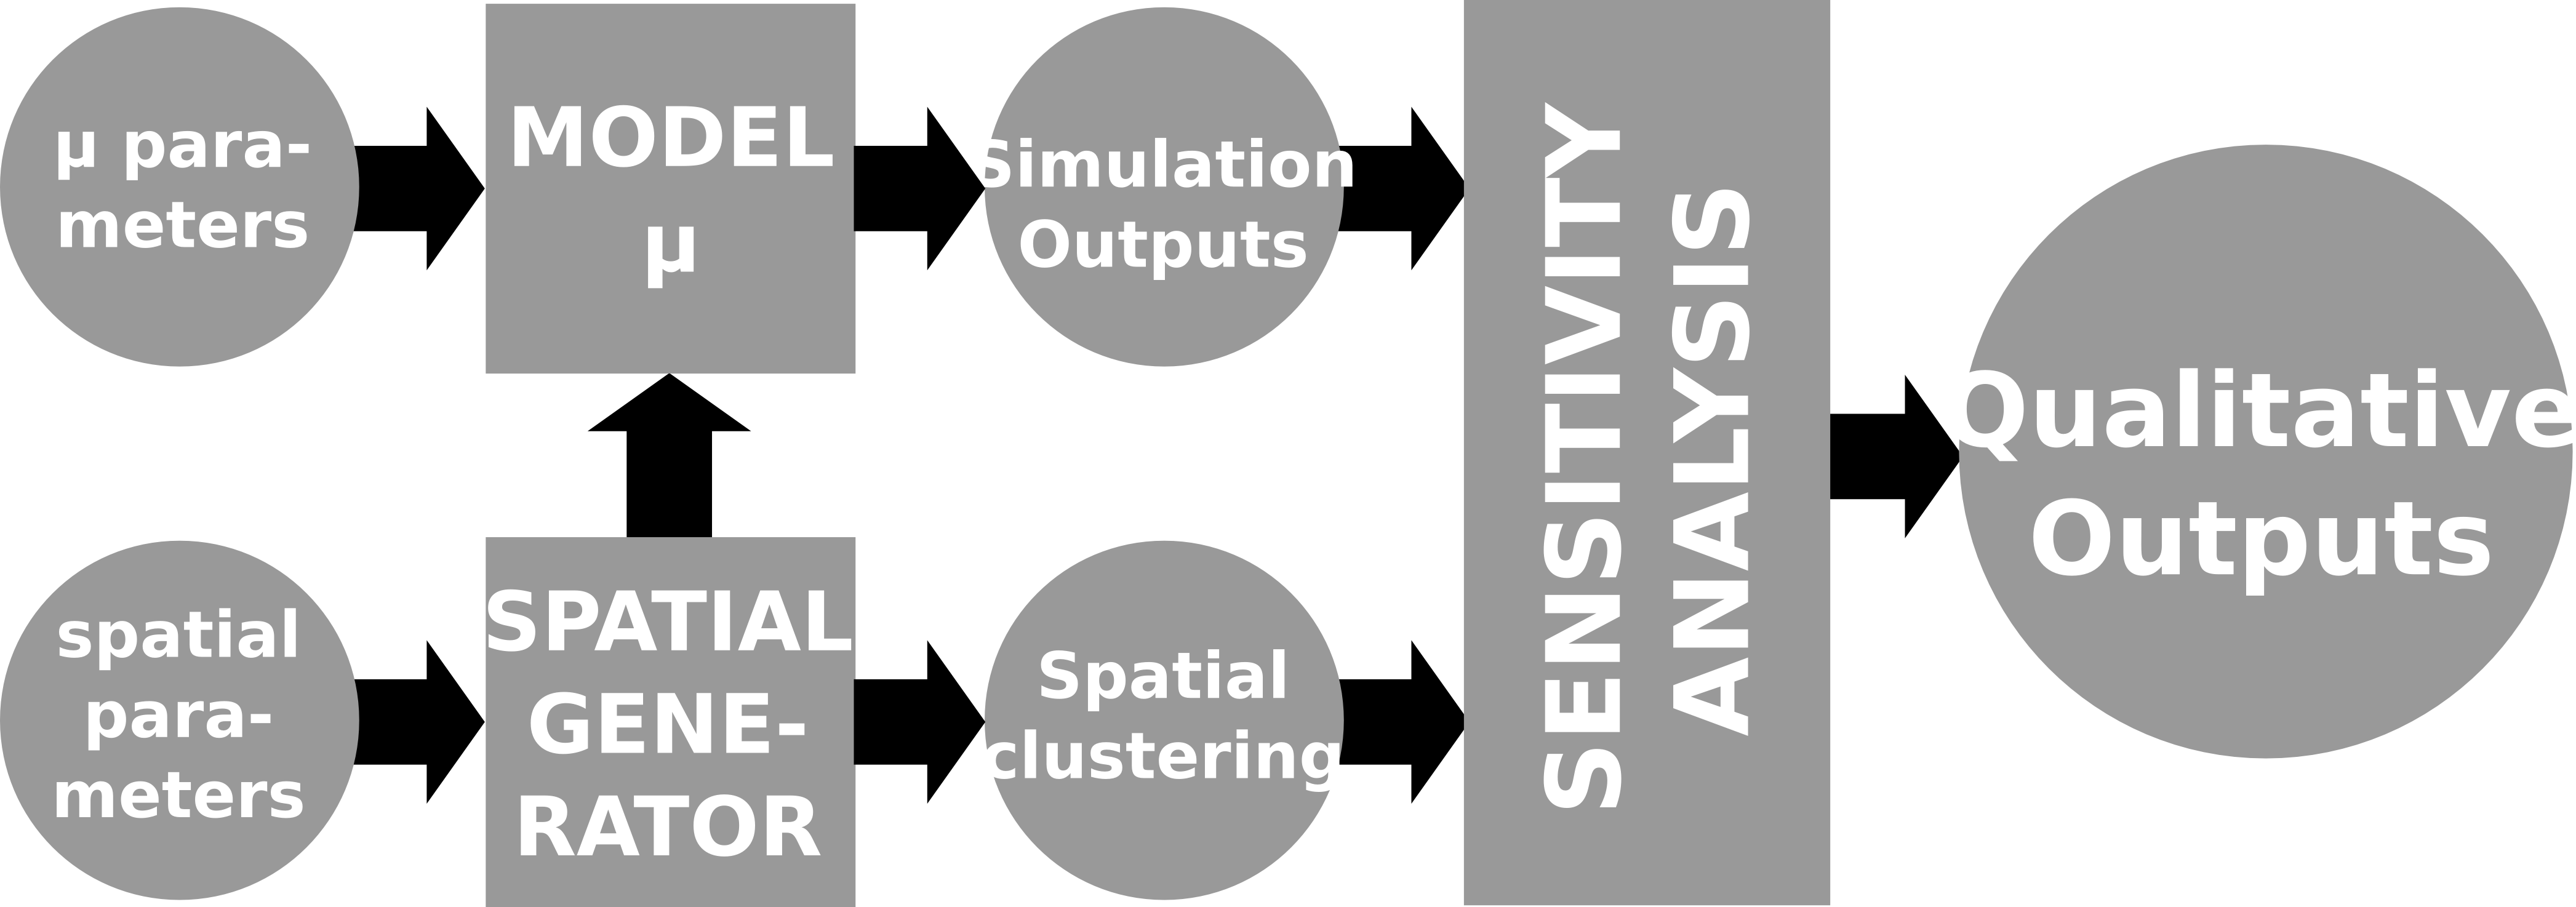
\includegraphics{figures/SchemaMeta_1.png}
} \caption{\textbf{General workflow of our method.}} \label{fig:method} \end{center} \end{figure*} %
%%%%%%%%%%%%%%%%%%%%%%

In our approach, we introduce a spatial generator (lower branch in figure \ref{fig:method}), which itself is determined by input parameters and produces sets of spatial initial conditions. 
To allow for the exploration of the relative effects of model parameters and spatial configuration, we cluster initial spatial conditions  to represent types of spaces ex-ante (for example: monocentric or polycentric density grids). The sensitivity analysis of the model is now run against $\mu$ parameters as well as spatial parameters or spatial types. It allows the sensitivity analysis to produce qualitative conclusions regarding the influence of spatial distribution on the outputs of simulation models, alongside the classic variation of parameter values.

In order to test for the influence of spatial initial conditions on model outputs, we use a systematic method to compare phase diagrams. We define a phase diagram as the vector of model outputs considered as a function of model parameters. Technically, because of stochasticity, we represent the output of the model for a given combination of parameter values as the median of the final values of an output indicator obtained for the replications of the model initialized with this combination of parameters.\\

%Comparing phase diagrams is useful because it allows us to compare the 
Indeed, we have as many phase diagrams than we have spatial grids, what makes a qualitative visual comparison not realistic (with around 50 different spatial configurations in our applications). A solution is to use systematic quantitative procedures. To our knowledge there exist no well established method to compare phase diagrams in agent-based modeling and geosimulation literature. We propose to use a relative distance between two phase diagram corresponding to the share of between-diagrams variability relative to their internal variability, given formally in the case of a one-dimensional phase diagram by

%\comment[FL]{je ne comprends pas ce choix : pourquoi faut il considérer que des classes ayant une forte cohérence interne seraient plus éloignées? ou alors la question ne se pose pas en ces termes... Par ailleurs est ce que la formule est bien homogène du point de vue des dimensions? En tous cas je pense qu'on peut se passer de la formule à ce stade, éventuellement à mettre dans l'affichage des résultats si on en a besoin.}[(JR) pour l'homogénéité oui justement on prend $d^2$ car c'est les variances, on obtient une mesure sans unité ; ok pour omettre la formule ; pour l'interprétation, on regarde la distance relative, pour des classes à une certaine distance, si elles sont concentrées, cette distance sera plus sigificative que si elles ont une grande variabilité et peuvent se recouper ; par exemple si elles ont mêmes variance $\sigma^2$, alors si $d \simeq \sqrt{2} \sigma$ alors les nuages de points vont en gros se recouper sur leur moitié (cas gaussien idéal), tandis que si $d\gg \sigma$, le max d'un diagramme sera très loin du min de l'autre - on compare à la fois la distance relative et la distance de forme.]

%Several potential methods from other fields such as environmental science could be used, but we keep it simple and such methodological considerations are furthermore auxiliary to the main purpose of this paper. We propose therefore an intuitive measure corresponding to the share of between-diagrams variability relative to their internal variability. More formally, the distance is given by

\begin{equation}\label{eq:phase-distance}
d_r\left(\vec{\alpha_1},\vec{\alpha_2}\right) = 2 \cdot \frac{d(f_{\vec{\alpha_1}},f_{\vec{\alpha_2}})^2}{Var\left[f_{\vec{\alpha_1}}\right] + Var\left[f_{\vec{\alpha_2}}\right]}
\end{equation}

where $f_{\vec{\alpha_i}}$ are the phase diagrams at given meta-parameters $\vec{\alpha_i}$. $d$ is a functional distance that we take simply as Euclidian distance. The variances are estimated within each phase diagram $f_{\vec{\alpha_i}}$. For a multi-dimensional phase diagram, we sum these relative distances over the components. 


The last methodological point which we need to emphasis is the relation between the workflow we introduce and model exploration workflows. The ideas of multi-modeling and extensive model exploration are nothing from new as ~\cite{openshaw1983data} already advocated for ``model-crunching'', but their effective use only begins to emerge thanks to the apparition of new methods and tools together with an explosion of computation capabilities. The model exploration platform OpenMole~\citep{reuillon2013openmole} allows to embed any model as a blackbox, write modulable exploration workflow using advanced methodologies such as genetic algorithms and distribute transparently the computation on large scale computation infrastructures such as clusters or computation grids. In our case, the workflow tool is a powerful way to embed both the sensitivity analysis and the meta-sensitivity analysis, and allow to couple any generator with any model in a straightforward way as soon as the model can take its spatial configuration as input or from an input file. In this paper, we use the OpenMole platform for spatial environment and model coupling, placing ourselves in the renewed framework of multi-modelling claimed by \citet{cottineau2015modular}.
%%%%%%%%%%%%%%%%%%%%%%
\subsection{Spatial generator of density grids}

The spatial generator applies an urban morphogenesis model \citep{Batty2007}, which has been generalised, explored and calibrated by~\citet{2017arXiv170806743R}. An open implementation and a characterisation of urban forms the model can produce are provided, what allows us to integrate it easily in our workflow. In a nutshell, grids are generated through an iterative process which, starting from a void grid, adds a quantity $N$ (population) at each time step $t$, allocating it through preferential attachment on population density, characterised by its strength of attraction $\alpha$. More precisely, each added unit has a probability equal to $P_i^{\alpha}/\sum_k P_k^{\alpha}$ to be added to patch $i$ with population $P_i$, all $N$ units being added independently and in parallel. At the end of each time step, this growth process is smoothed $n_d$ times using a diffusion process of strength $\beta$: each patch transmits an equal share of $\beta\cdot P_i$ to its extended neighborhood (8 surrounding patches). To avoid border effects such as a reflexion on the border of the world, border patches diffuse to the outside. The procedure stops when a fixed number of steps $t_f$ is reached. The grid then has a population of $t_f \cdot N$ (the population lost due to diffusion process to the outside is reallocated through a normalization procedure at the end of the steps). Grids are thus generated from the combination of the values of these four meta-parameters $\alpha$, $\beta$, $n_d$ and $N$, in addition to the random seed. To ease our exploration, only the distribution of density is allowed to vary rather than the size of the grid, which we fix to a 50x50 square environment. We furthermore fix the total population at $t_f\cdot N = 100,000$, and determine therein the number of steps needed at a given $N$. Typical value ranges for the  parameters will be taken as, following \citet{2017arXiv170806743R}, $\alpha\in\left[0.5,4.0\right]$, $\beta \in\left[0,0.3\right] $, $N\in \left[100,10000\right]$, $n_d\in\left[1,4\right]$. We illustrate in Fig.\ref{fig:spatialGen} the variety of spatial configuration that can be generated.

%\comment[MLT]{Il me semble que l'on pourrait mieux expliciter la relation N/n (et peut-être du coup inverser N et n). Plus il me semble que l'on devrait dire plus clairement à quoi se réfère alpha : à une cellule $i$? au pas de temps $t$? Pourquoi ne pas indexer alpha? Enfin, je crois que l'on gagnerait encore plus en clarté si on expliquait formellement comment tous les paramètres sont reliés entre eux, notamment pour expliquer l'arrêt de la procédure d'attribution d'une nouvelle pop à la grille.} \comment[FL]{je crois que N c'est l'incrément de pop et n le nombre de fois où c'est smoothé mais c'est quoi la pop totale?}



%%%%%%%%%%%%%%%%%%%%%%
\begin{figure*}[htbp] \begin{center} 
\resizebox{0.9\textwidth}{!}{ 
	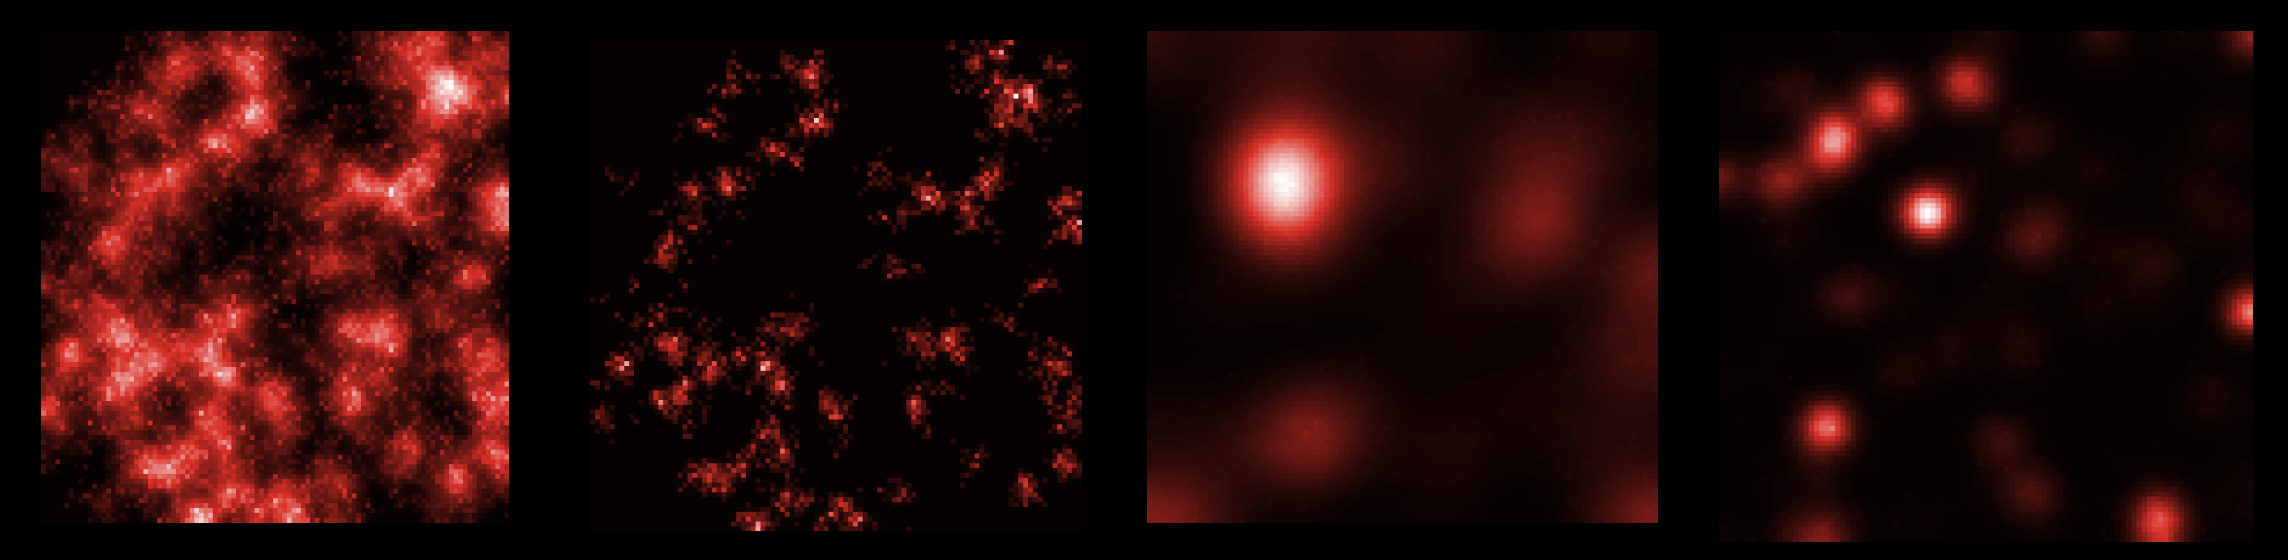
\includegraphics{figures/spatialGen.png}
} \caption{Four examples of grids produced by the spatial generator. The lighter the red, the denser the area. Changing the growth rate $N$ allows to have more or less chaotic shapes (two first compared to the two last grids for example) corresponding to different levels of convergence of the model, whereas local radius can be tuned with the interplay of aggregation strength $\alpha$ and diffusion strength $\beta$.} \label{fig:spatialGen} \end{center} \end{figure*} %
%%%%%%%%%%%%%%%%%%%%%%

%%%%%%%%%%%%%%%%%%%%%%
\begin{figure*}[htbp] \begin{center} 
\resizebox{0.9\textwidth}{!}{ 
	\includegraphics{figures/GridPresentation.png}
} \caption{Correspondence between European urban density structures and grids produced with the spatial generator.} 
\label{fig:densityTypes} \end{center} \end{figure*} %
%%%%%%%%%%%%%%%%%%%%%%



%%%%%%%%%%%%%%%%%%%%%%
%\subsection{Including a (typical) variety of initial conditions in the sensitivity analysis}

In order to generate density grids which correspond to empirical density distributions, we select among the generated grids using an objective function which matches the point cloud of 110 metropolitan areas in Europe described by four dimensions of spatial structure : their concentration index, hierarchy index, centrality index and continuity index (cf. \cite{LeNechet2015}). We sample the meta-parameter space using a Latin Hypercube Sampling, which is a convenient technique to have a point cloud with high discrepancy. We sample 2000 points in the 4-dimensional space of parameters {$\alpha$, $\beta$, $n$, $N$}. It yields a subset of 170 interesting grids matching empirical densities, which constituted our set of different initial spatial conditions. These are further clustered into three classes of morphology: compact (e.g. Vienna), polycentric (Liege) and discontinuous (Augsburg) in order to evaluate the non-trivial effects of urban form on simulation results. We select 15 grids of each type to work with in the computation of sensitivity analysis, obtaining a total of 45 spatial configurations to compare (as we will see, the significant number of model runs needed to establish each phase diagram imposes a computational limit on this number of configurations).

%\comment[FL]{pourquoi 15?} \comment[FL]{dire explicitement ce qu'on va faire avec ces catégories dans la partie résultats?}





In the following section, we briefly recall the main components of the two ``classical'' agent-based simulation models used to test how spatial density variations may impact simulation models behaviour and results, and how general the method proposed is.

\subsection{Case study models}


Schelling's model consists in an abstract urban housing market where agents of different nature sense their environment, evaluate their satisfaction in terms of neighbourhood composition, and relocate if unsatisfied. It has been shown by \cite{Schelling1969} that even tolerant agents tended to produce segregated patterns because of the complexity of their local interactions. The main parameters of this model are the tolerance level (\% of agents similar to {\it ego}), the scope of sensing and the percentage of vacant spaces in the housing market. In addition, we are interested in testing the impact of the spatial distribution of housing capacity in this project, using the generated grids. The outcome of the model is measured as a phase diagram of segregation level, described by the combination of several indicators: Dissimilarity, Moran's Index, Entropy~\citep{brown2006spatial}.

Sugarscape is a model of resource extraction which simulates the unequal distribution of wealth within a heterogenous population \citep{EpsteinAxtell1996}. Although it {\it "is designed to study the interaction of many plausible social mechanisms"} \citep[p.125]{Axtelletal1996}, we refer in this paper to the first (and simplest) version of the model, where {\it "processes allow its agents to look for, move to, and eat a resource ("sugar") which grows on its toroidal array of cells"}. Agents of different vision scopes and different metabolisms harvest a self-regenerating resource available heterogeneously in the initial landscape, they settle and collect this resource, which leads some of them to survive and others to perish. The main parameters of this model are the number of agents, their minimal and maximal resource. In addition, we are interested in testing the impact of the spatial distribution of the resource in this project, using the generated grids. We extend the implementation with agents wealth distribution of~\citet{li2009netlogo}. The outcome of the model is measured as a phase diagram of an index of inequality for resource distribution (Gini index). 


\subsection{Experiment design}
For Schelling's model, we explore a grid of a basic parameter space of the model, which is composed of two dimensions: the minimum proportion of similar agents required in the neighbourhood for the agent to be satisfied (or intolerance level) $S\in \left[0;1\right]$ and the vacancy rate of the city $V\in \left[0;1\right]$, which then defines the number of green and red agents, present in equal proportion for this experiment. We sample 1000 parameter values using a Sobol sampling and run 100 repetitions for each configuration. The initial spatial configuration varies across 45 different grids, chosen among the ones which are most representative of the three types of urban morphology: 15 compact grids (like Vienna, cf figure \ref{fig:densityTypes}), 15 polycentric grids (like Liege) and 15 discontinuous grids (like Augsburg). The full experiment thus equates to 4,500,000 simulations (1000 parameter combinations x 45 density grids x 100 replications). We use OpenMOLE to distribute the computation, and apply segregation measures to characterise the results.

For Sugarscape, we explore a grid of a basic parameter space of the model, which is composed of three dimensions: the population of agents $P\in \left[10;510\right]$, the minimal initial agent resource $s_{-}\in \left[10;100\right]$ and the maximal initial agent resource $s_{+}\in \left[110;200\right]$. Each parameter is binned into 10 values, giving 1000 parameter points. We run 50 repetitions for each configuration, what yield reasonable convergence properties. The initial spatial configuration varies across 50 different grids, generated by sampling meta-parameters for the generator in a LHS. We did not use the clustered grids to test the flexibility of our framework, which is demonstrated in this case by a direct sequential coupling of the generator and the model. Indeed, because the density distribution refers to the distribution of resource rather than to the representation of a city structure, we do not need the typology of urban density in this experiment. The full experiment thus equates to 2,500,000 simulations (1000 parameter combinations x 50 density grids x 50 replications). 


We choose different design of experiments, both for meta-parameters and for the phase diagram, to demonstrate the robustness of the method to technical choices. In principle, our workflow applies with any manner to generate a spatial configuration (even taking real configurations) and any manner to establish phase diagrams.




%%%%%%%%%%%%%%%%%%%%%%
\section{Results}
%%%%%%%%%%%%%%%%%%%%%%

%\comment[FL]{il faudrait peut être davantage renforcer l'analyse a propos de figure 1 de si c'est plutôt les mu parameters ou les spatial parameters qui ont une grosse influence sur les résultats.}[(JR) assez explicite pour sugarscape, j'ai rajouté un peu tout de même.]

\subsection{Quantitative variation across grids}



\paragraph{Sugarscape} We measure the distance of all phase diagrams to the reference phase diagram computed on the default model setup, which is a bi-centric symmetric configuration (see Fig.~\ref{fig:sugarscape-distance-meta} for its morphological positioning regarded generated grids), using the relative measure defined in equation~\ref{eq:phase-distance}. Indeed, it gives in that case the average squared distance between corresponding points of the phase diagrams, relative to the average of the variance of each. Therefore, values greater than 1 will mean that inter-diagram variability is more important than intra-diagram variability.


% summary stats
%   Min. 1st Qu.  Median    Mean 3rd Qu.    Max. 
% 0.08909 0.19790 1.52200 1.29600 2.16400 2.98100 

We obtain a very strong sensitivity to initial spatial conditions. Indeed, the relative distance of phase diagrams of different density grids to the reference case ranges from 0.09 to 2.98 with a median of 1.52 and an average of 1.30. The mean distance above 1 means that, on average, the model is more sensitive to meta-parameters of grid generation than to its own parameters (population and sugar). Moreover, the maximum distance of 2.98 means that the variation due to the change of grid can be 3 times bigger than the variation due to the model's parameters. We plot in Fig.~\ref{fig:sugarscape-distance-meta} the distribution of these distances in a morphological space. Each point represent one of the 50 different density grids used to initialised the distribution of sugar in the model. The points are projected with respect to the meta-parameters used to generate the grid, and coloured according to the relative distance of the phase diagram of the simulations using this grid to the phase diagram of the reference case. Therefore, the figure ~\ref{fig:sugarscape-distance-meta} shows that the grids generated with a high $\alpha$ (i.e. with a small number of very high density cells) produce simulation results more different compared to the reference case than within this reference case because of parameter variations. This pattern is emphasized when grids are generated with a high $\alpha$ AND a high $\beta$ (i.e. with low gradient of density decrease around the kernels of high density). These grids have the highest relative distance to the reference case. On the contrary, with grids closer to random and uniform patterns (bottom left of the graph), the model's parameters are more important in determining the simulation results. 


%%%%%%%%%%%%%
\begin{figure}
\centering
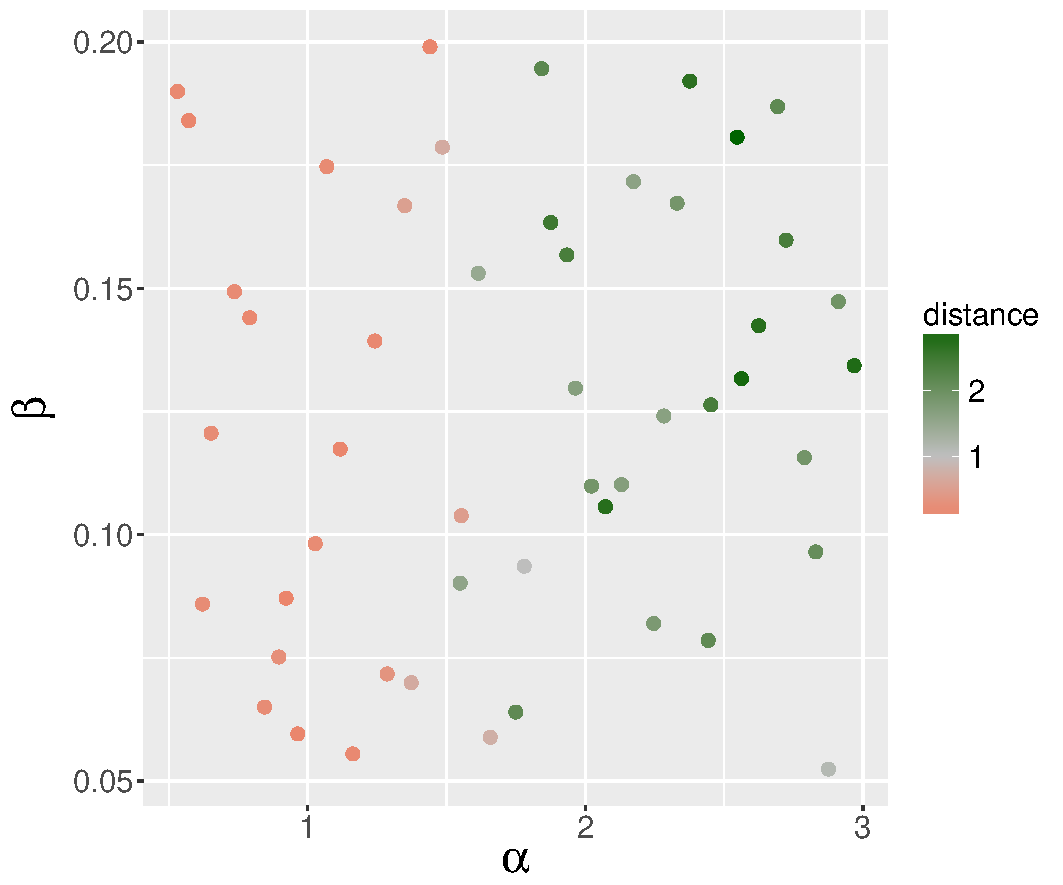
\includegraphics[width=0.8\textwidth]{figures/relativedistance_metaparams}\\
%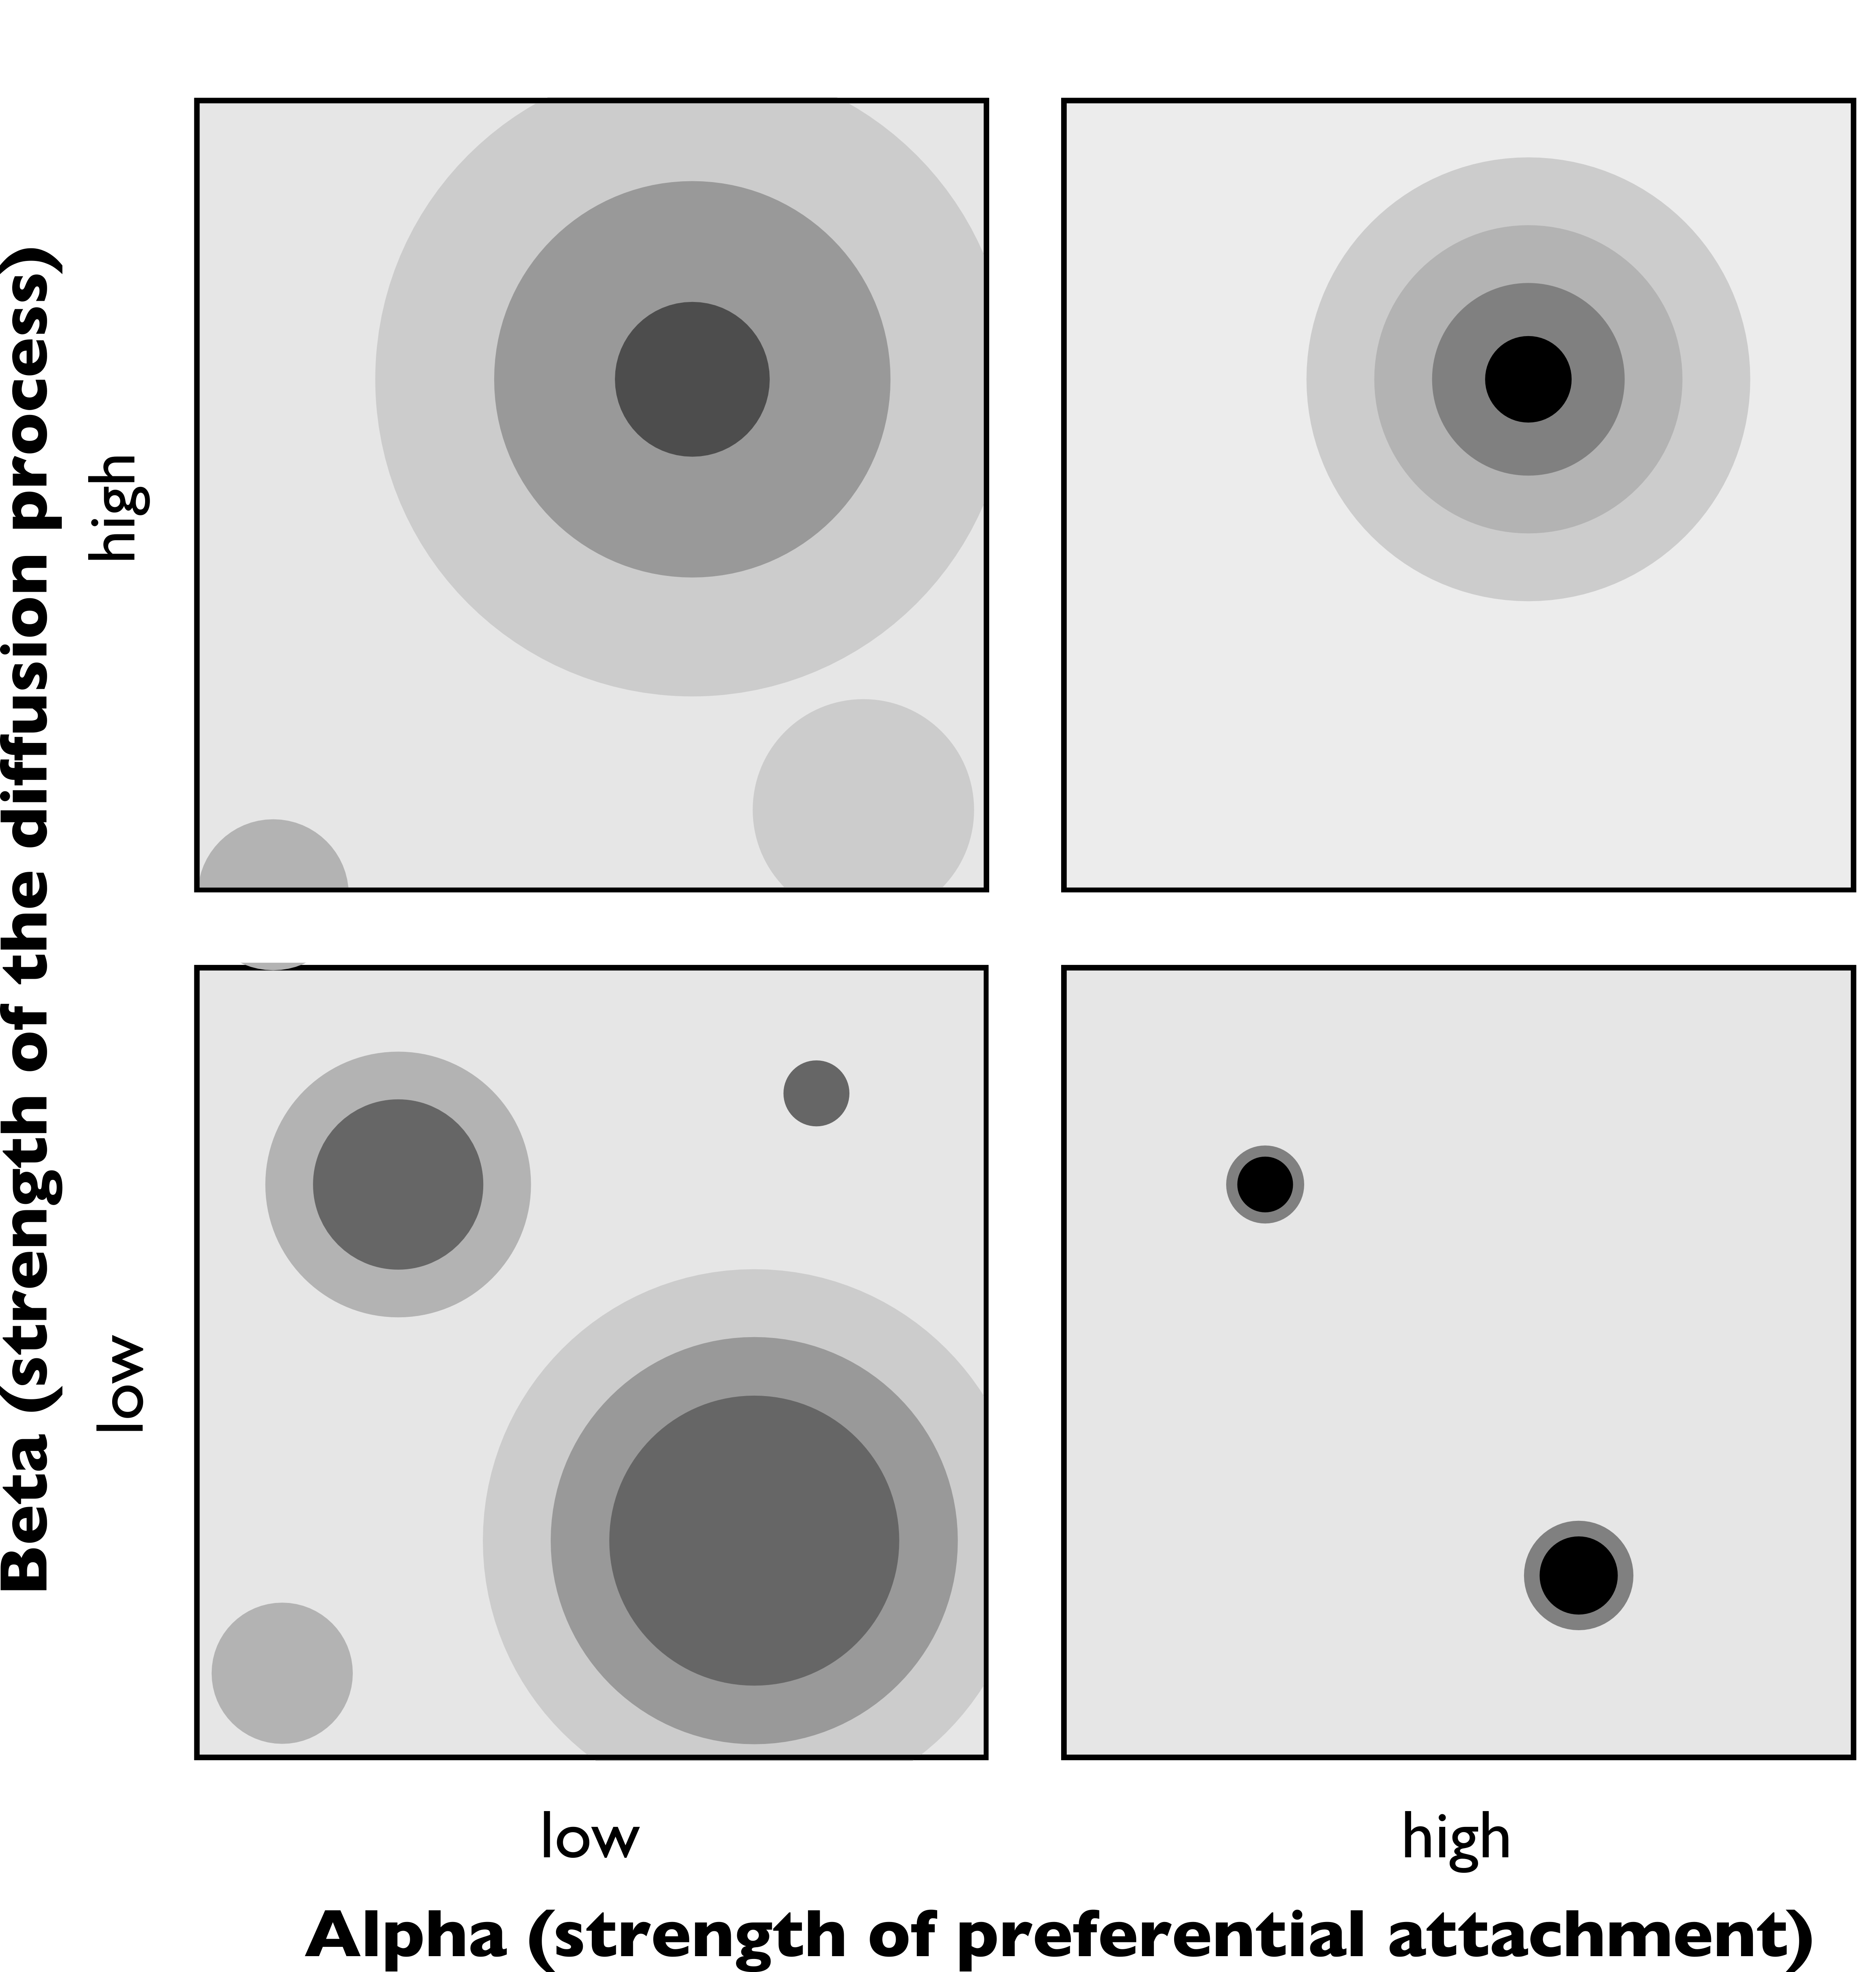
\includegraphics[width=0.4\textwidth]{figures/alpha_beta_schemas}(Bottom) Corresponding stylised density grids\\\comment[JR]{je sais pas si c'est une bonne idee de mettre les grilles stylisees comme ca parce que ca donne une fausse idee des sorties du modele de generation}}
\caption{\textbf{Relative distances of phase diagrams by initial spatial grids described by the meta-parameters of their generator.} Relative distance as a function of meta-parameters $\alpha$ (strength of preferential attachment) and $\beta$ (strength of diffusion process).}
\label{fig:sugarscape-distance-meta}
\end{figure}
%%%%%%%%%%%%%

Another way of quantifying the density grids, instead of looking at the meta-parameters of their generator, is to look at the resulting indicators of urban form, such as Moran index, average distance, rank-size slope and entropy (see~\cite{LeNechet2015} for precise definition and context). This 4-dimensional space defined a morphological space. For the purpose of interpretability and visualisation, we reduce this space to a bi dimensional space with a principal component analysis. The first two components represent 92\% of cumulated variance. The first component defines a ``level of sprawl'' and of scattering, whereas the second one represents the level aggregation.\footnote{We have $PC1 = 0.76\cdot distance + 0.60\cdot entropy + 0.03\cdot moran + 0.24\cdot slope$ and $PC2 = -0.26\cdot distance + 0.18\cdot entropy + 0.91\cdot moran + 0.26\cdot slope$.} We find that grids producing the highest deviations are the ones with a low level of sprawl and a high aggregation (top left of figure \ref{fig:sugarscape-distance-pca}). It is confirmed by the behavior as a function of meta-parameters, as high values of $\alpha$ also yield high distance. In terms of model processes, it shows that congestion mechanisms in the gathering of the resource induce fast increases of inequality. To put these results in perspective of our work-flow given in Fig.~\ref{fig:method}, we have a sensitivity to spatial parameters in average greater than the sensitivity to model parameters.


% pca of morphological space
% "","PC1","PC2","PC3","PC4"
%"distance",0.762358566609464,-0.260991693298744,0.200656405132039,0.557162237616392
%"entropy",0.601306167355116,0.181706245959277,0.0958379422351422,-0.772158547261002
%"moran",0.0311129390452153,0.912155429075071,0.30114271129527,0.276256268103684
%"slope",0.237217819823539,0.258531718397015,-0.927289147645628,0.130475642169329

%%%%%%%%%%%%%
\begin{figure}
\centering
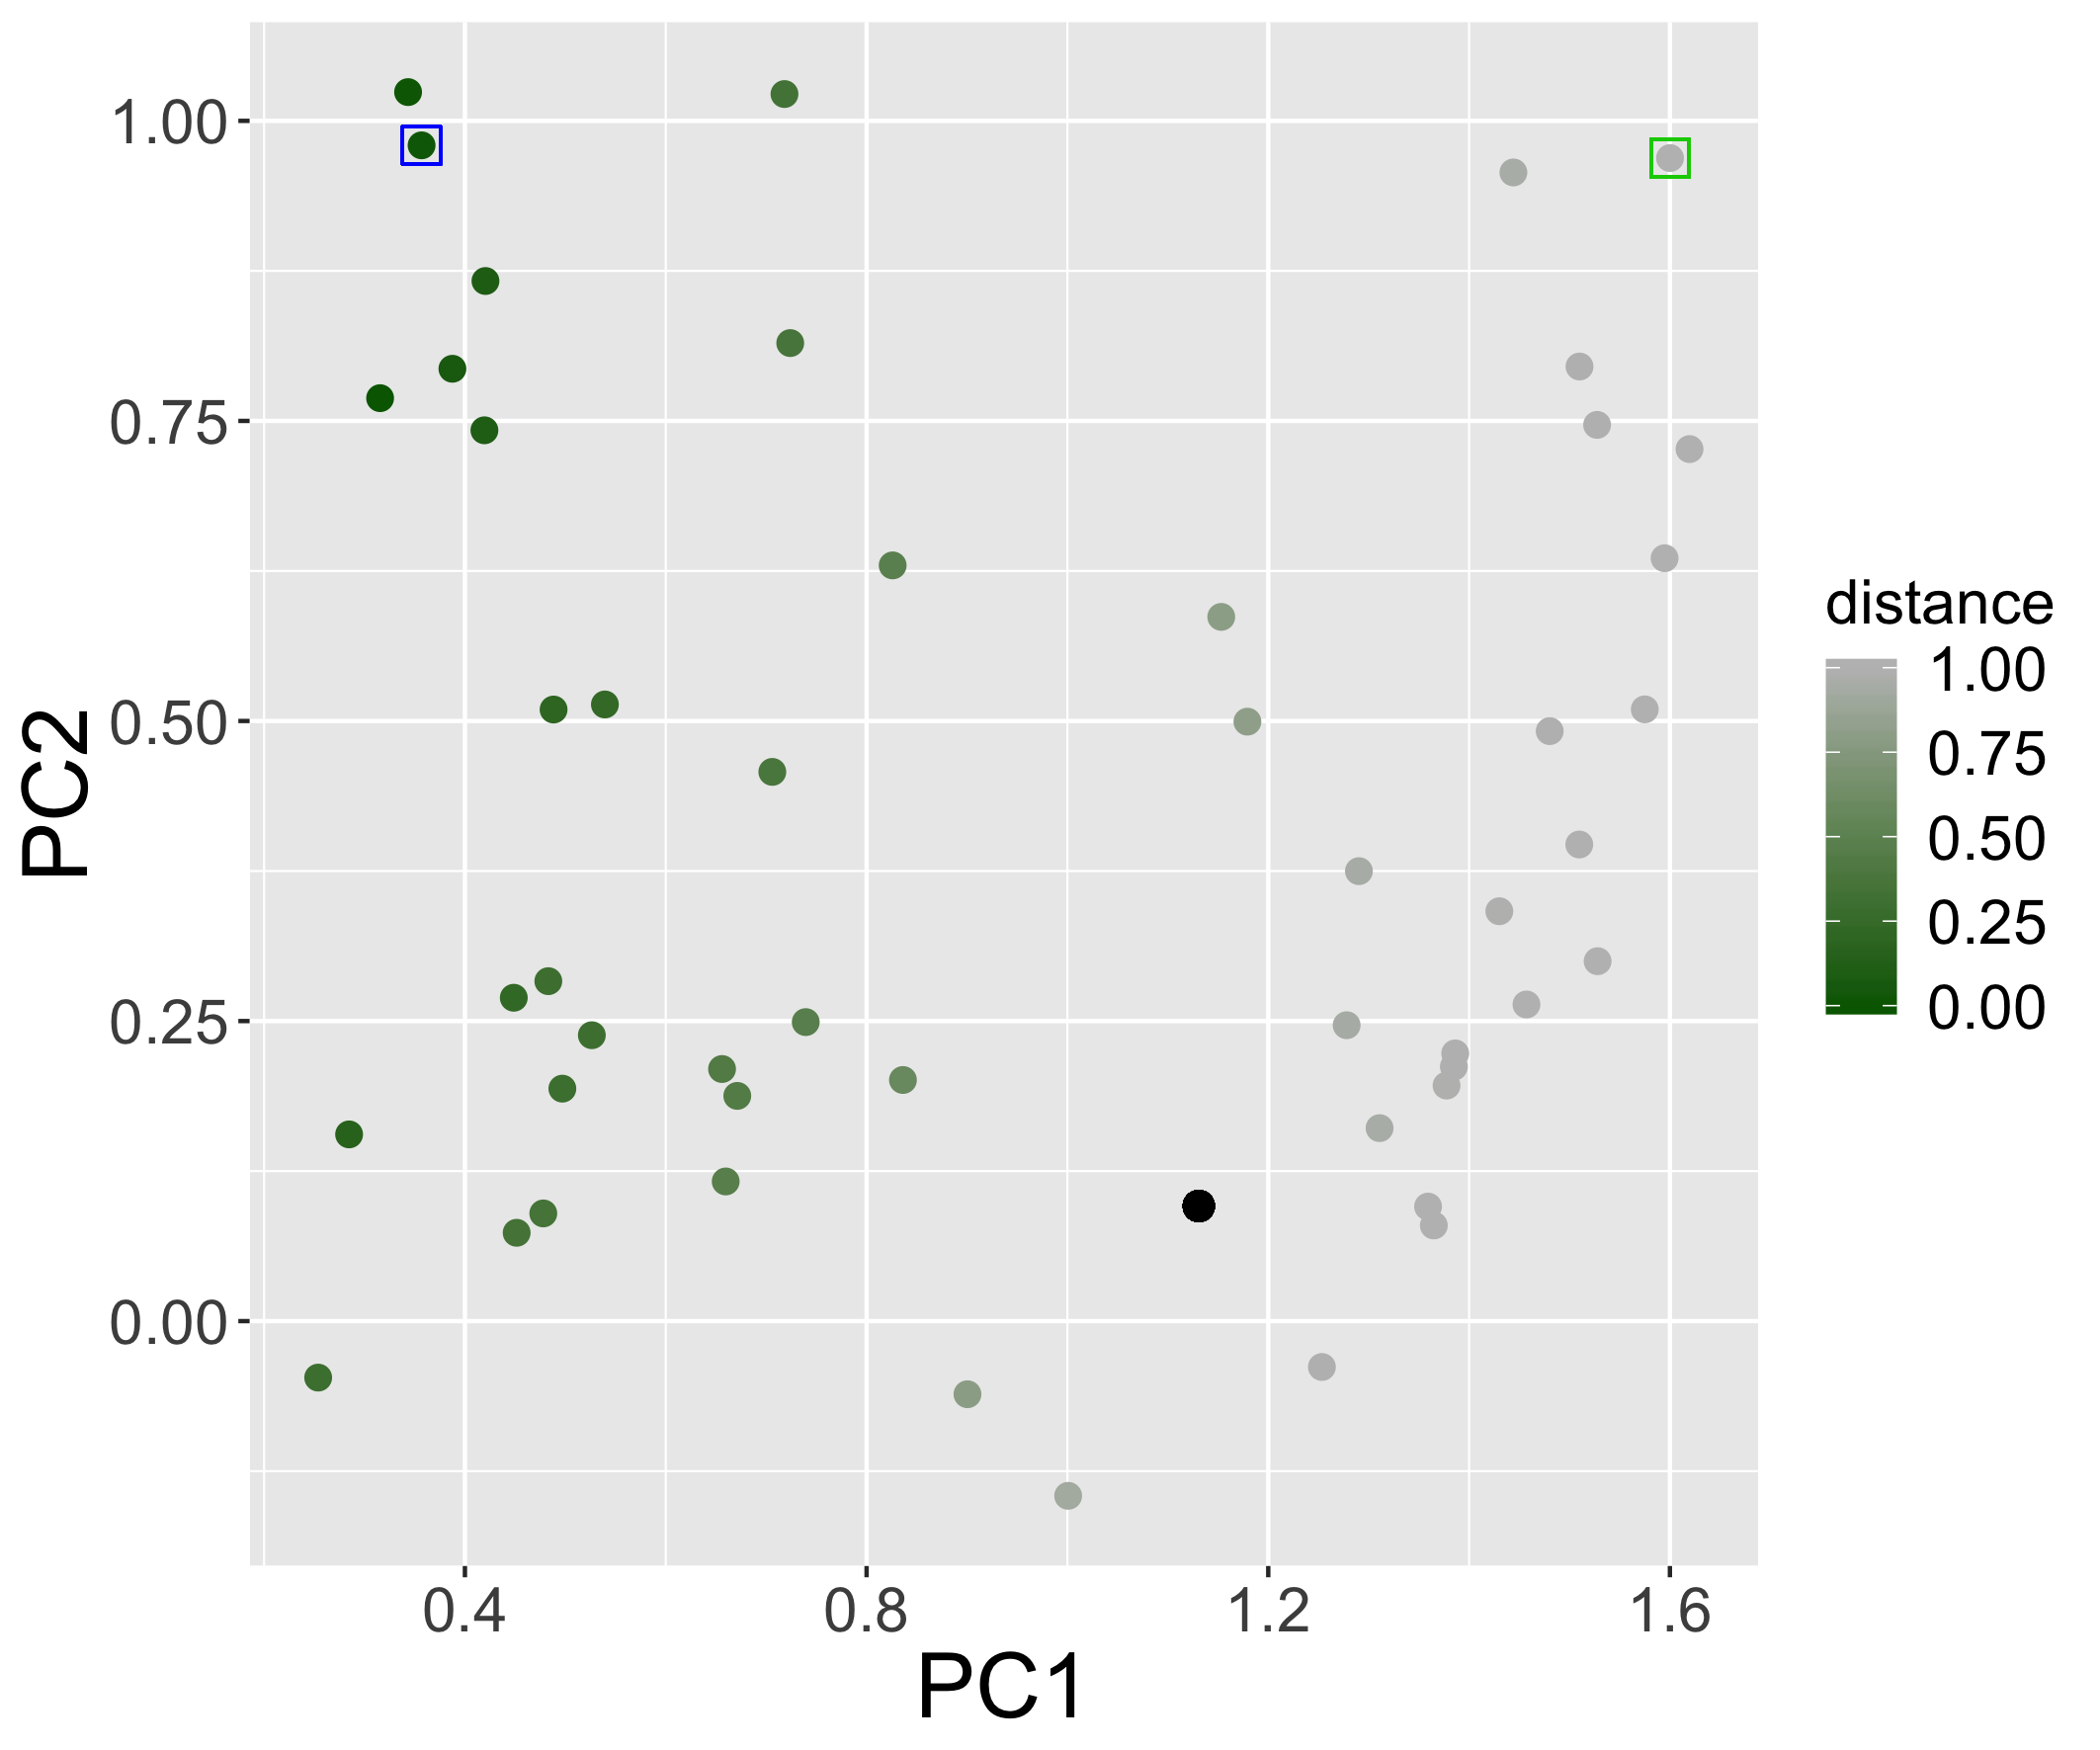
\includegraphics[width=0.8\textwidth]{figures/relativedistance_morphspace}
\caption{\textbf{Relative distances of phase diagrams to the reference across grids.} Relative distance as a function of two first principal components of the morphological space (see text). Black point correspond to the reference spatial configuration. Green frame and blue frame give respectively the first and second particular phase diagrams shown in Fig.~\ref{fig:sugarscape-phasediagrams}.}
\label{fig:sugarscape-distance-pca}
\end{figure}
%%%%%%%%%%%%%



\paragraph{Schelling} 
Within a standard Schelling model (i.e. initialised with a uniform density grid), \citet{Gauvinetal2009} have built the phase diagram of segregation patterns depending on the combination of parameter values. For high levels of tolerance ($S < 0.25$), there is no segregation. For high values of vacancies ($V > 0.65$) and low values of tolerance ($S > 0.5$), these is a diluted segregation state where homogeneous communities are separated from other by large empty buffers. Finally, for low values of vacancies ($V < 0.2$) and low values of tolerance ($S > 0.7$), the model is frozen in a state where everyone is unhappy but no-one can express their intolerant behaviour due to the lack of free spaces. Between these extreme cases, the model gives rise to segregated states where homogeneous communities adjoin one another. The objective of this quantitative experiment is to evaluate to which extent this phase diagram is modified when different density grids are applied. We show in Fig.\ref{fig:schelling-distance-meta} the values of the relative distance as a function of meta-parameters and in the reduced morphological space, in a way similar to the analyse done with Sugarscape before. Variations are less considerable than for Sugarscape across phase diagrams, but values close to 1 show that several configurations are as much sensitive to space than to their parameters. We will focus in the following in a qualitative characterisation of variations.


%%%%%%%%%%%%%
\begin{figure}
\centering
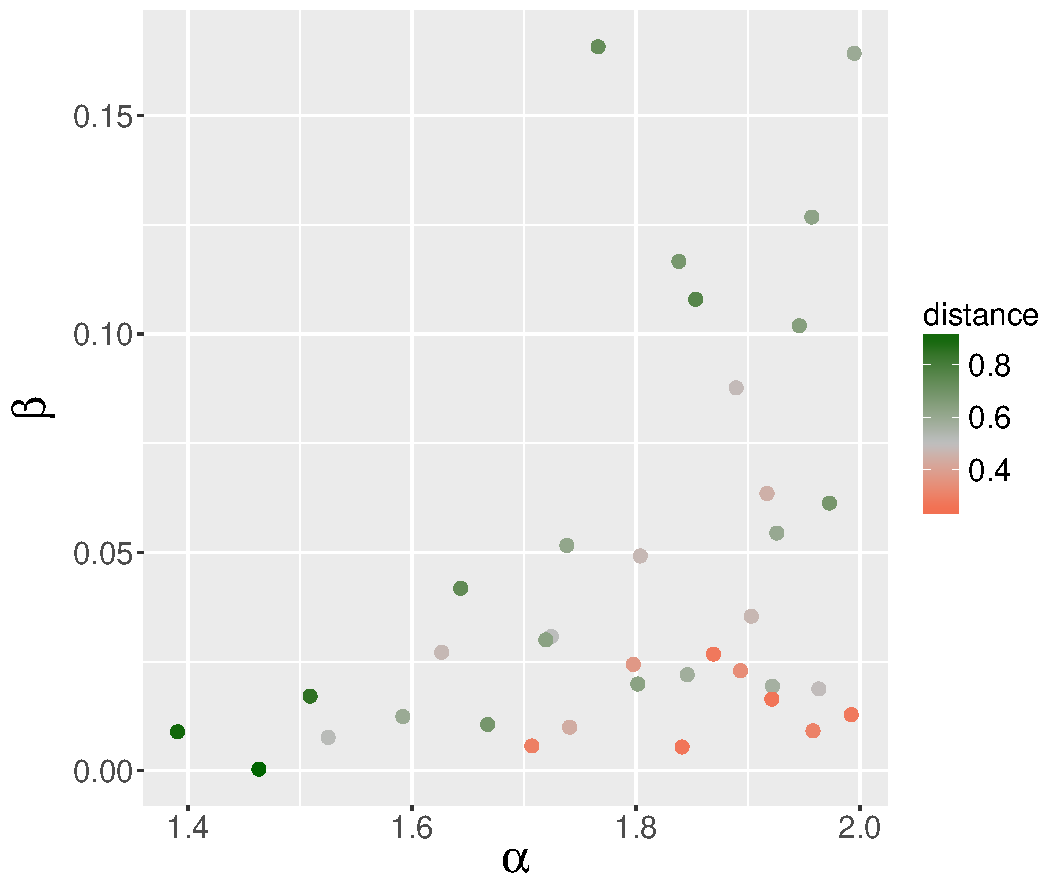
\includegraphics[width=0.48\textwidth]{figures/schelling-relativedistance_metaparams}
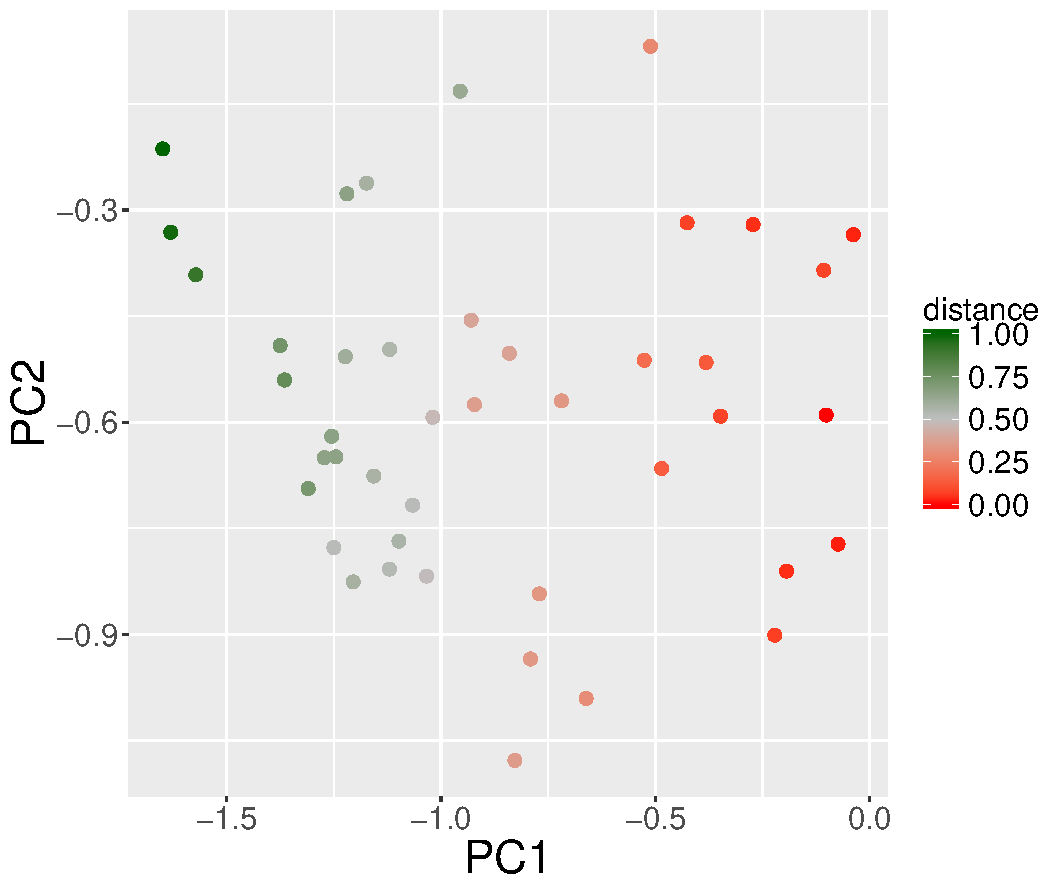
\includegraphics[width=0.48\textwidth]{figures/schelling-relativedistance_morphspace}
\caption{\textbf{Relative distances of phase diagrams to the reference across grids for the Schelling model.} Each point corresponds to a spatial configuration and colour gives the relative distance to one of the phase diagrams. We show them in the meta-parameter space (Left) and in the reduced morphological space (Right).\label{fig:schelling-distance-meta}}
\end{figure}
%%%%%%%%%%%%%





\subsection{Qualitative variations}
\paragraph{Sugarscape} We now check the sensitivity in terms of qualitative behavior of phase diagrams. We show the phase diagrams for two very opposite morphologies in term of sprawling, but controlling for aggregation with the same $PC2$ value. These correspond to the green and blue frames in Fig.~\ref{fig:sugarscape-distance-pca}. The behaviors are rather stable for varying $s_+$, what means that the poorest agents have a determinant role in trajectories. The two examples have not only a very distant baseline inequality (the ceiling of the first 0.35 is roughly the floor of the second 0.3), but their qualitative behavior is also radically opposite: the sprawled configuration gives inequalities decreasing as population decreases and decreasing as minimal wealth increases, whereas the concentrated one gives inequalities strongly increasing as population decreases and also decreasing with minimal weights but significantly only for large population values. The process is thus completely inverted, what would have significant impacts if one tried to schematise policies from this model. To interpret these behavior in terms of grid shape, we observe that the difference between the two grids is mainly on average distance and entropy: in a nutshell, the first grid is much more dispersed and disorganised than the second. In sprawled spaces, inequalities are thus fostered by a lack of minimal local ressources, whereas population will drive inequality in concentrated spaces.

%This second example confirms thus the importance of sensitivity of simulation models to the initial spatial conditions.


% phase diagrams -> ok well different qualitatively
%          spAlpha spDiffsteps spDiffusion spGrowth spPopulation
% id=27 : 0.7913103    2.376837   0.1440293 157.4147 4852.746
% id=0 : 2.562398    3.753032   0.1316788 128.4632 4753.983
% maxSugar = 110


%%%%%%%%%%%%%
\begin{figure}
\centering
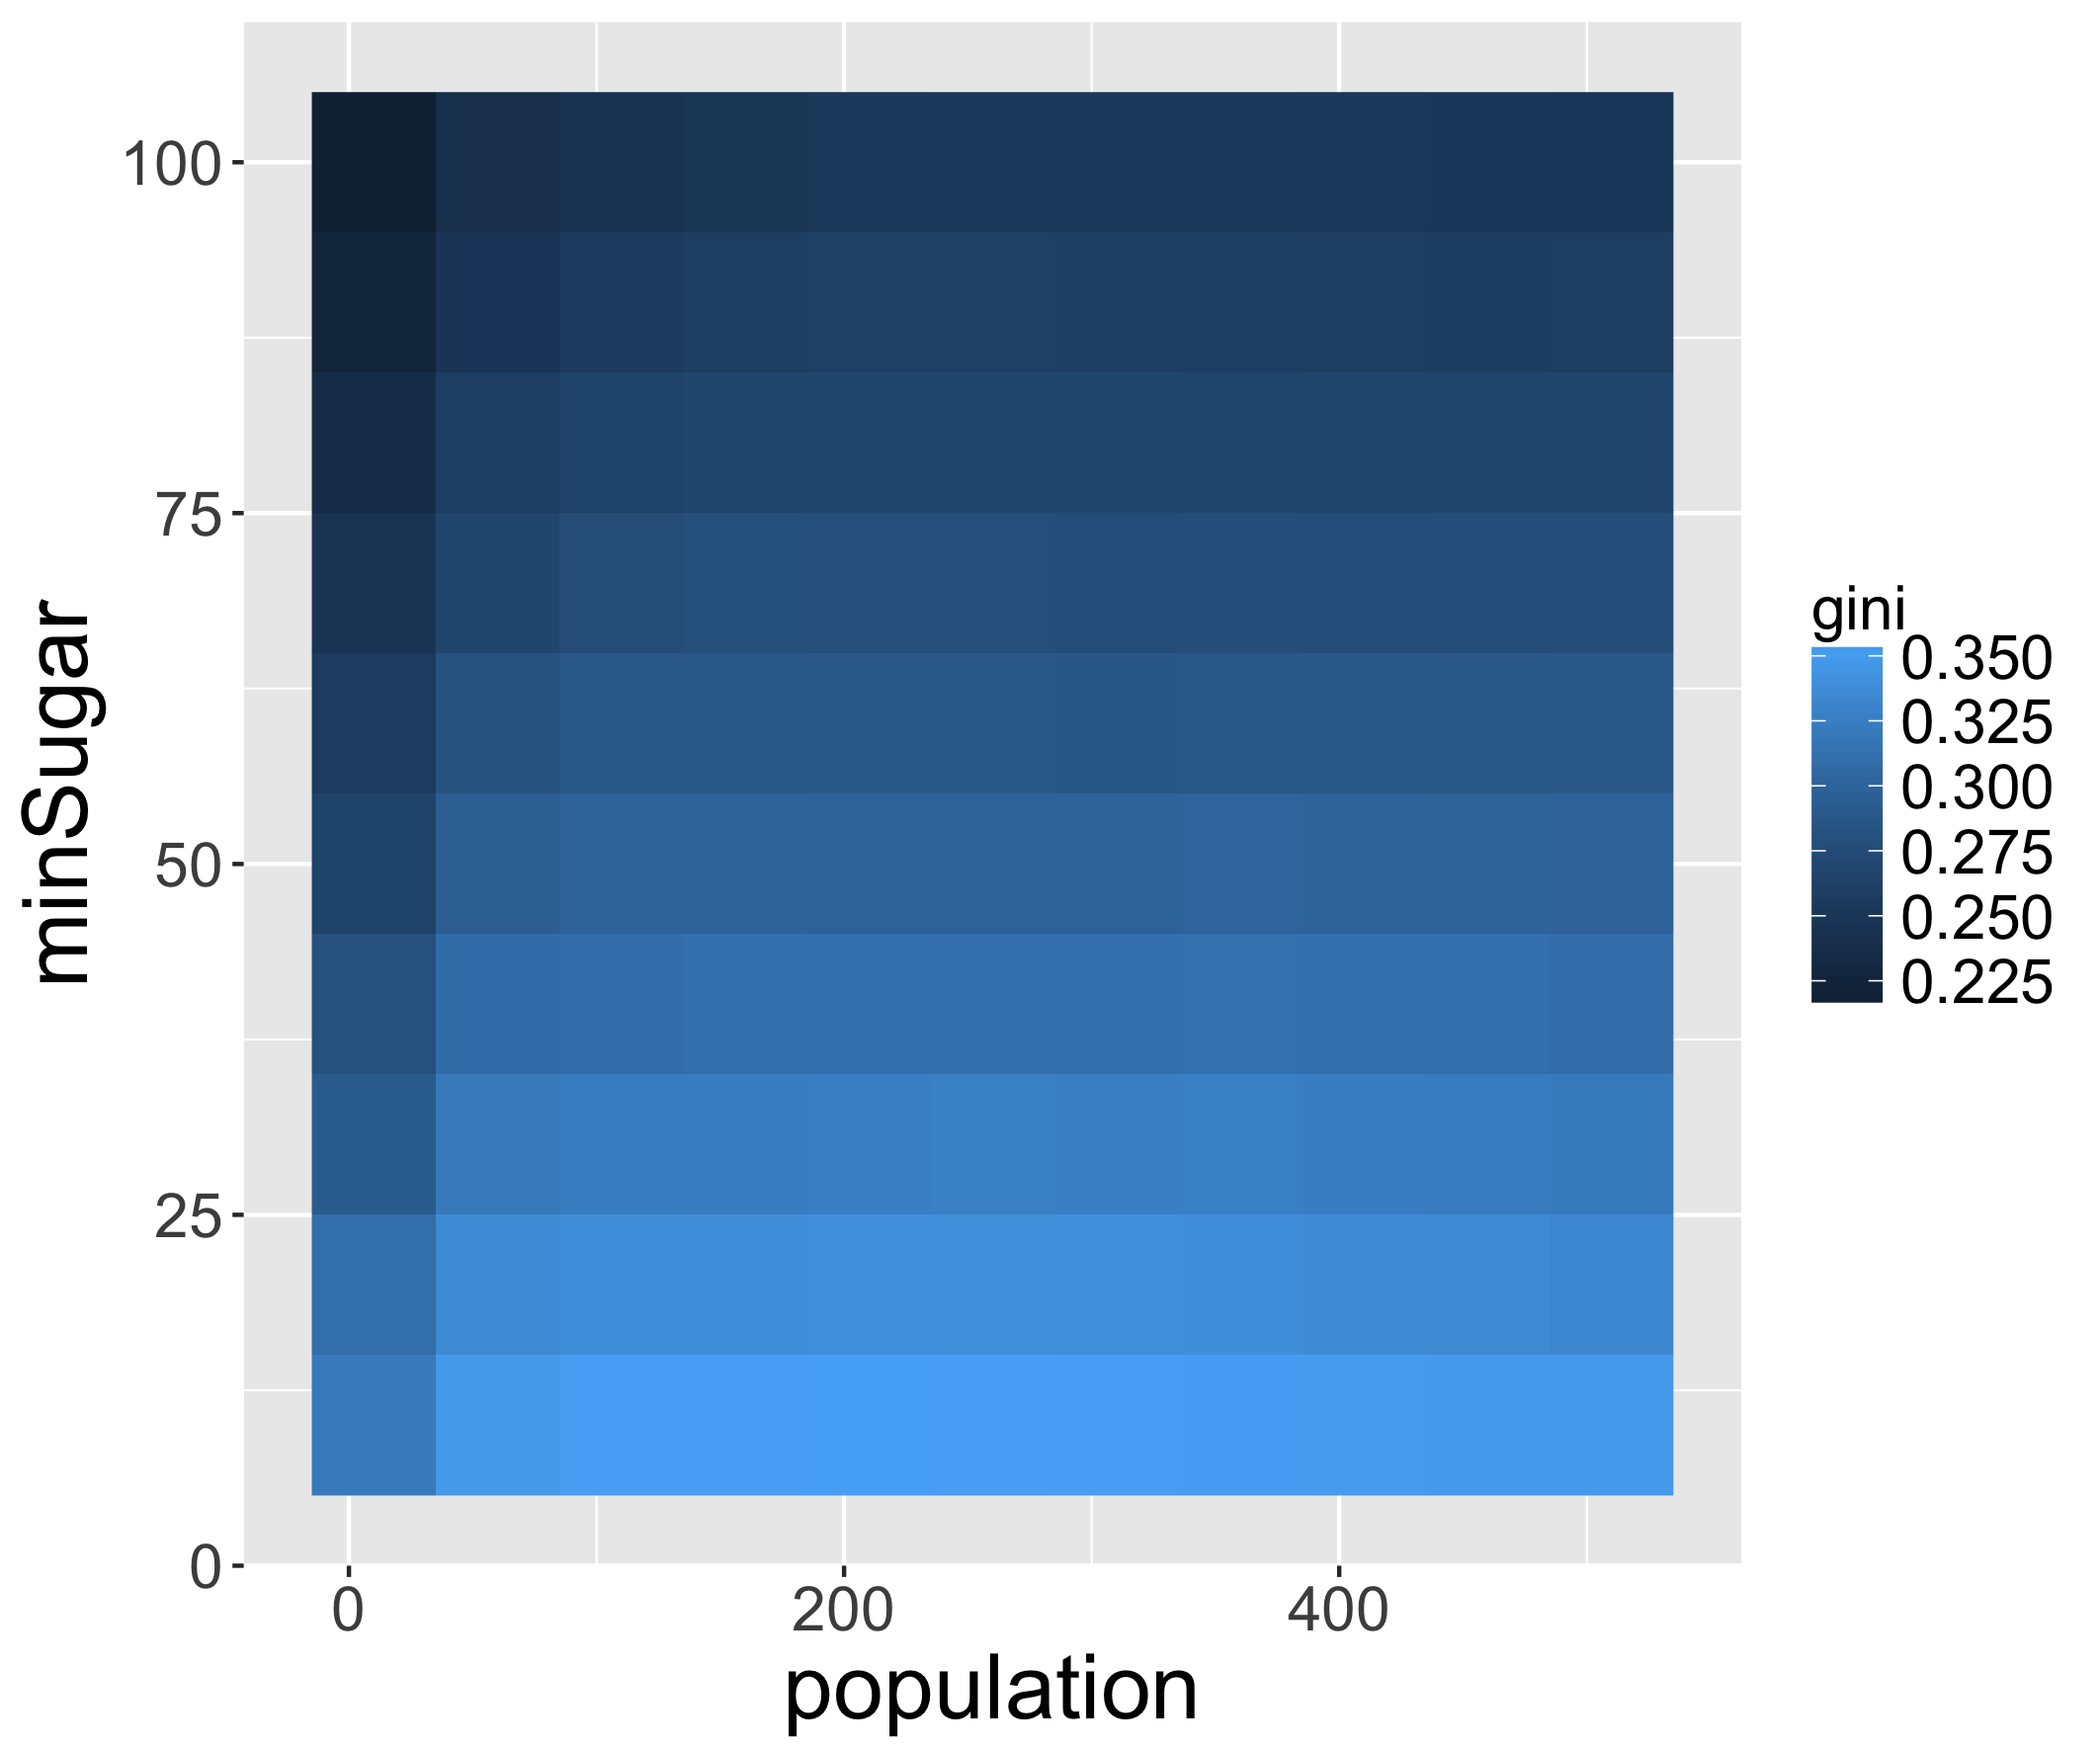
\includegraphics[width=0.48\textwidth]{figures/phasediagram_id27_maxSugar110}
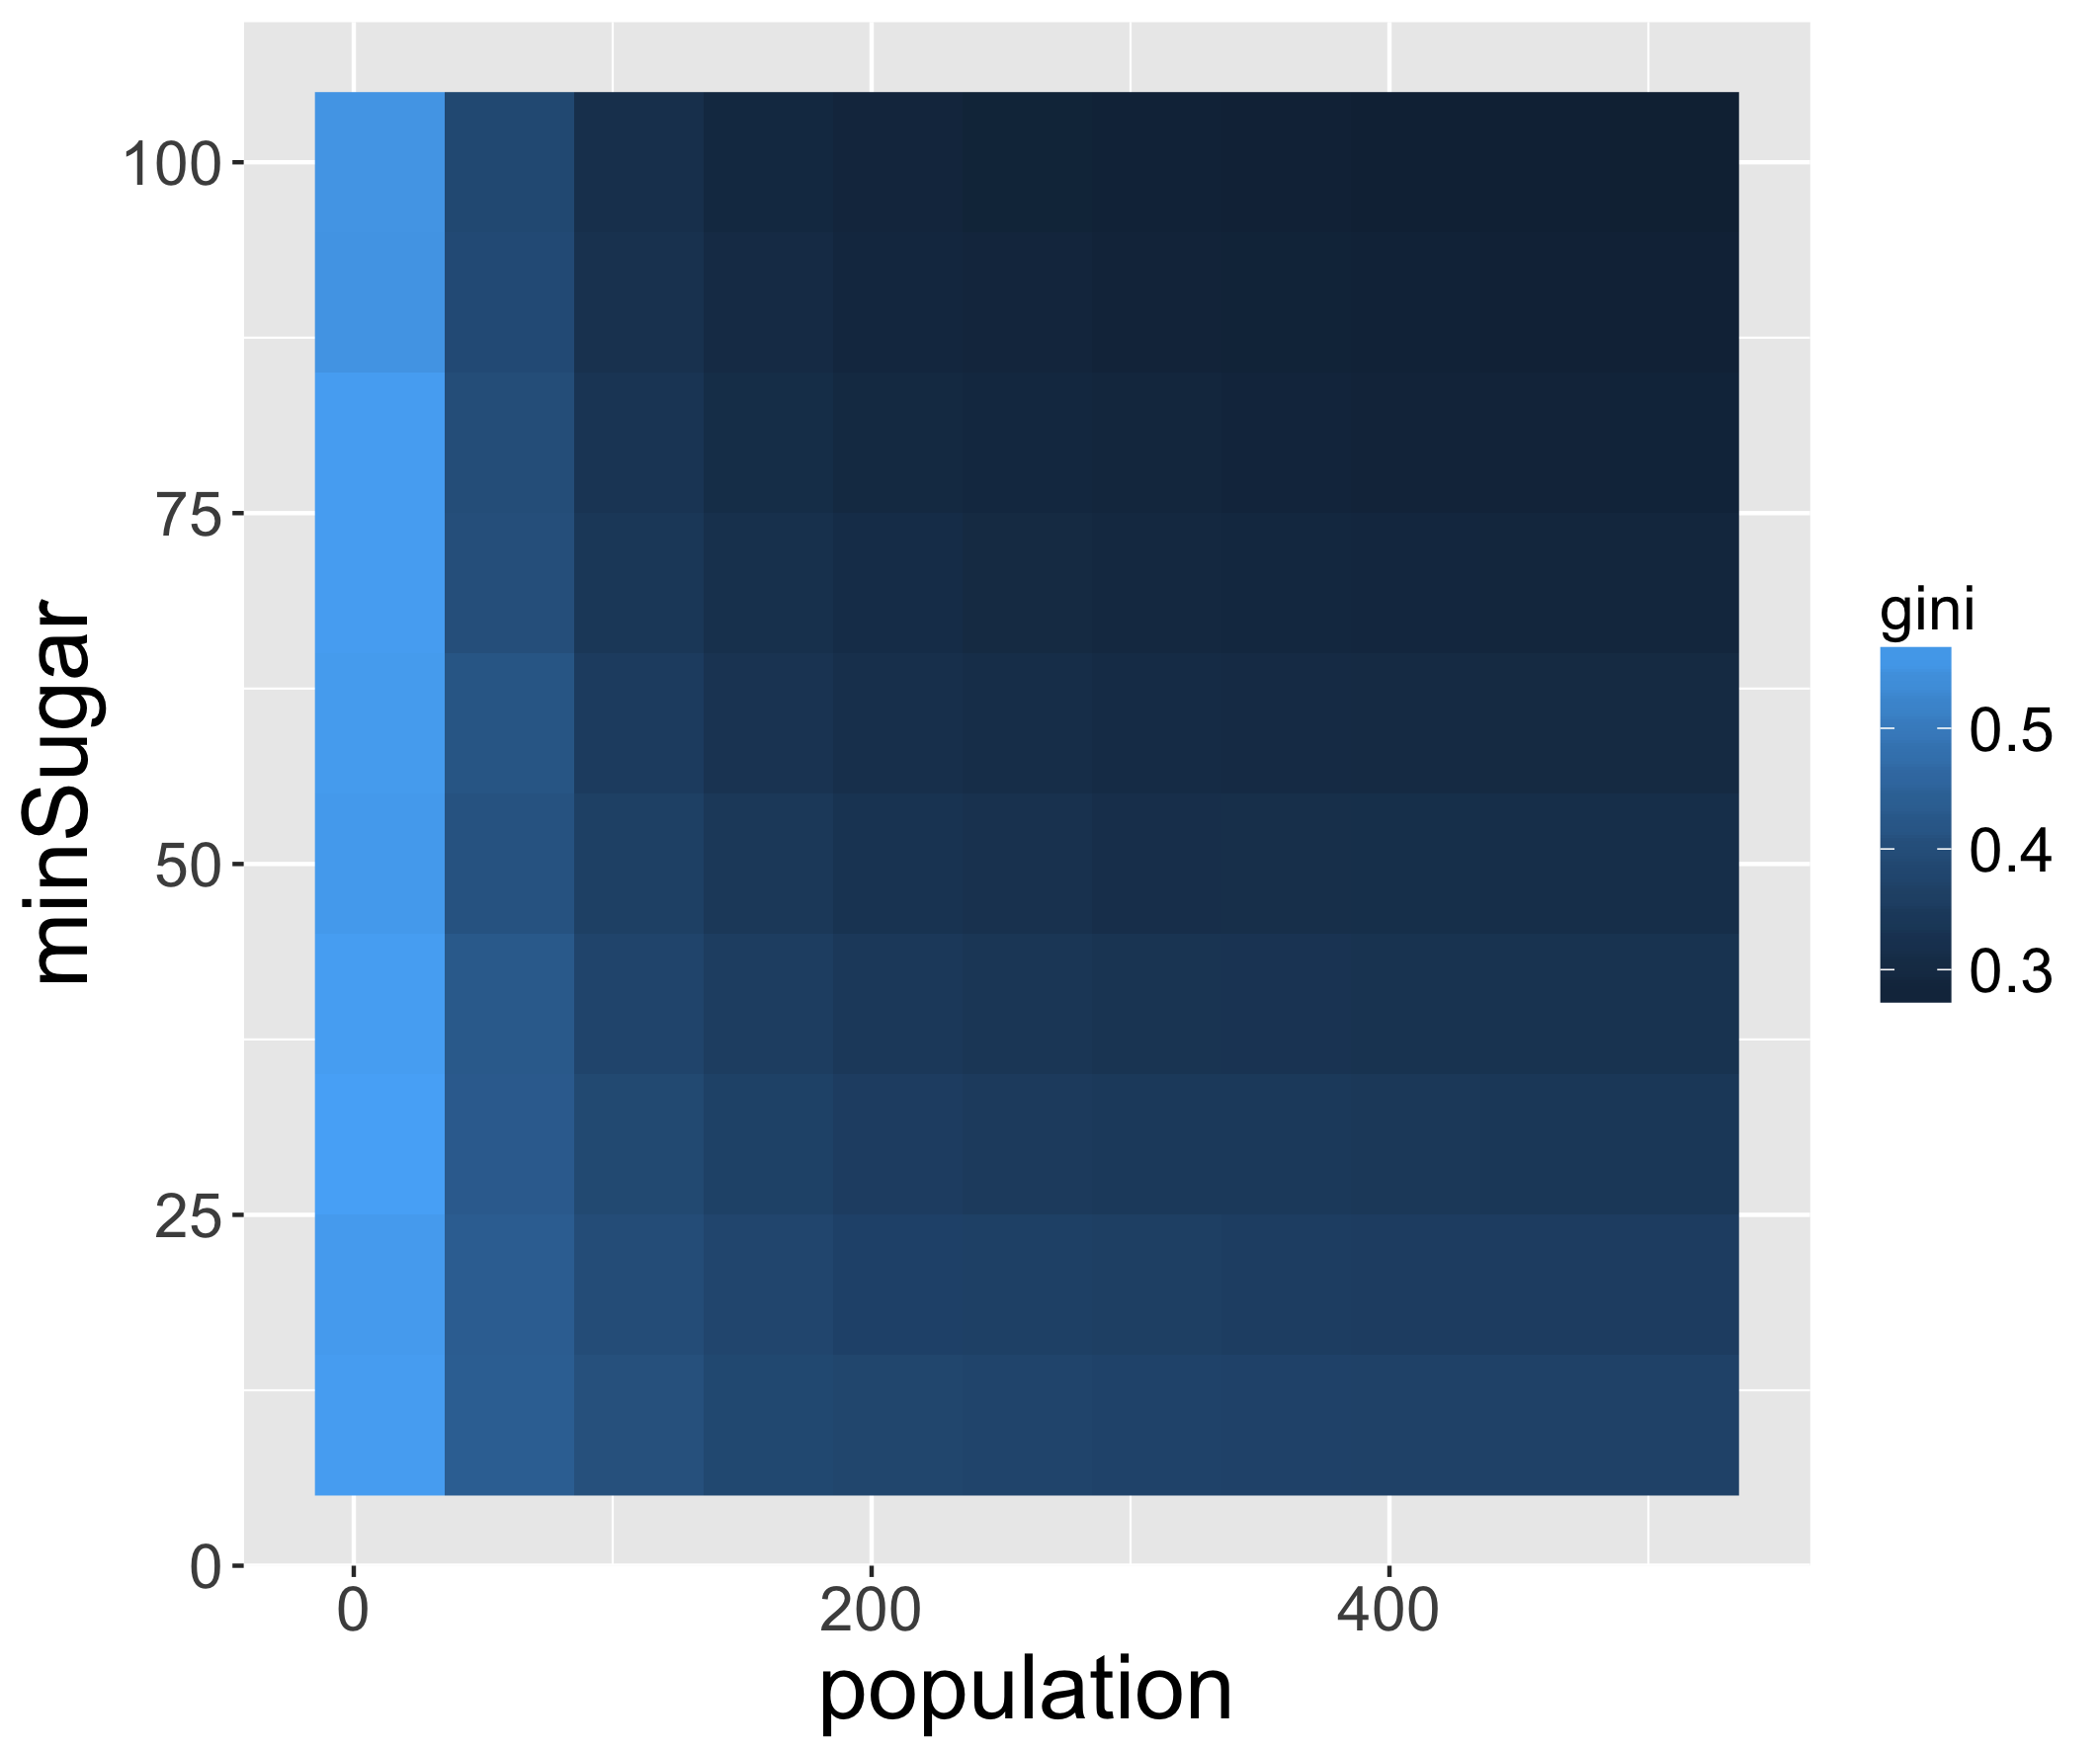
\includegraphics[width=0.48\textwidth]{figures/phasediagram_id0_maxSugar110}
\caption{\textbf{Examples of phase diagrams.} We show two dimensional phase diagrams on $(P,s_-)$, both at fixed $s_+ = 110$. (Left) Green frame, obtained with $\alpha = 0.79$, $n=2$, $\beta = 0.14$, $N=157$; (Right) Blue frame, obtained with $\alpha = 2.56$, $n=3$, $\beta = 0.13$, $N=128$.}
\label{fig:sugarscape-phasediagrams}
\end{figure}
%%%%%%%%%%%%%




\paragraph{Schelling} In this qualitative exploration of the effect of initial spatial conditions on the results of Schelling's model, we use the classification of grids into three morphological types (cf. figure \ref{fig:densityTypes}). In particular, we want evaluate to which extent the typology summarises the spatial effects, and so if one type of urban form or the other enhances or mutes the segregation mechanism of the model, or interacts differently with the model parameters. This experiment aims at suggesting topical conclusions on urban morphology, beyond the technical conclusions already obtained with respect to simulation sensitivity.





\begin{table*}[]
\centering
\caption{\textbf{Regression of the segregation level of Schelling simulation with order parameters and type of city grid.} *** means that the estimate is significant at the 0.01 level.}
\label{tab:regressionSchelling}
\begin{adjustwidth}{-1cm}{-1cm}
\begin{tabular}{|m{2.5cm}|ll|ll|ll|}
\hline
Simulation outcome by segregation index:    & \multicolumn{2}{c|}{\textbf{Dissimilarity}}   & \multicolumn{2}{c|}{\textbf{Entropy}} & \multicolumn{2}{c|}{\textbf{Moran's I}} \\ \hline
\textbf{Intercept}                          & -0.212 *** & -0.141 ***                       & -0.254 ***        & -0.208 ***        & -0.036 ***           & -0.061 ***               \\ \hline
\textbf{Similarity Wanted (S)}              & 1.212 ***  & 1.212 ***                        & 1.250 ***         & 1.250 ***         & 0.550 ***            & 0.550 ***                \\ 
\textbf{quadratic term ($S^2$)}               & -0.942 *** & -0.942 ***                       & -0.963 ***        & -0.963 ***        & -0.428 ***           & -0.438 ***               \\ 
\textbf{Vacancy Rate (V)}                   & 0.602 ***  & 0.602 ***                        & 0.453 ***         & 0.453 ***         & -0.027 ***           & -0.027 ***               \\ 
\textbf{Minority Index (\%Maj - \%Min)}     & 0.307å ***  & 0.307 ***                        & 0.130 ***         & 0.130 ***         & -0.067 ***           & -0.067 ***               \\ \hline
\textbf{Density Grid = Polycentric}         &            & 0.087 ***                        &                   & 0.052 ***         &                      & 0.001 ***                \\ 
\textbf{Density Grid = Discontinuous}       &            & 0.111 ***                        &                   & 0.068 ***         &                      & \textit{0.00}              \\
\textbf{Attraction meta-parameter $\alpha$} &            & -0.083 ***                       &                   & -0.053 ***        &                      & 0.014 ***                \\ 
\textbf{Diffusion meta-parameter $\beta$}   &            & 0.323 ***                        &                   & 0.218 ***         &                      & 0.017 ***           \\ \hline
\textbf{R2 (\%)}                            & 30.6       & 34.7                             & 24.1              & 25.6              & 23.9                 & 24.0                    \\ 
\textbf{\# of observations (sim. runs)}     & 2,106,000  & 2,106,000 						 & 2,106,000          & 2,106,000          & 2,106,000             & 2,106,000                \\ 
\textbf{AIC}                                & -70717.68   & -198748.2  						& 208213.8          & 166048.8          & -4385990             & -4387816                 \\ \hline
\end{tabular}
\end{adjustwidth}
N.B. Moran's I applies to the minority population
\end{table*}

In table \ref{tab:regressionSchelling}, we see that the type of density grid with which the model is initialised determines to a certain extent the level of segregation measured at the end of the simulation run. Indeed, compared to compact density patterns, polycentric grids produce more dissimilarity and entropy between the location of green and red agents. Discontinuous grids have the same effect, although attenuated. The results obtained with Moran's I are opposite, because this index measures spatial autocorrelation at the global level and that compact cities have higher levels of global autocorrelation by construction. However, linear models with and without information about the type of density distribution yields the same coefficients for Schelling's parameters $V$ and $S$, the only exception being the vacancy rate $V$ in the Moran's I model with grid types, which becomes non-significant. The similarity of the coefficient in both cases means that the effect of the model's parameters (and thus the mechanism by which agents of similar group cluster in space) is the same regardless of the distribution of density. The way polycentric and discontinuous density grid exhibit higher segregation is by allowing buffer zones of low density to surround pockets of homogeneity, which is impossible in a compact city, because everyone is at reach of everyone else. The buffering process confirms previous results obtained with network structures \citep{Banos2012}.


%%%%%%%%%%%%%%%%%%%%%%
\section{Discussion}
%%%%%%%%%%%%%%%%%%%%%%

We consider that the method presented holds great potential for strengthening geographical models' validation. However, two limits and two areas of opportunities have still not been tackled. We discuss them in this section.

\subsection{Limits}

\paragraph{Comparing phase diagrams.} Comparing phase diagrams is as we saw not straightforward, and further developments of our method imply testing alternative methods for this particular point. For example in the case of the Schelling model, an anisotropic spatial segregation index (giving the number of clusters found and in which region in the parameter spaces they are roughly situated) would differentiate strong \emph{meta phase transitions} (phase transitions in the space of meta parameters). The use of metrics comparing spatial distributions, such as the Earth Movers Distance which is used for example in Computer Vision to compare probability distributions~\cite{rubner2000earth}, or the comparison of aggregated transition matrices of the dynamic associated to the potential described by each distribution, would also be potential tools. Map comparison methods, popular in environmental sciences %\comment[MLT]{Et pas en géo? Qu'est-ce que ces méthodes ont de particulier?}
, provide numeral tools to compare two dimensional fields~\cite{visser2006map}. To compare a spatial field evolving in time, elaborated methods such as Empirical Orthogonal Functions that isolates temporal from spatial variations, would be applicable in our case by taking time as a parameter dimension, but these have been shown to perform similarly to direct visual inspection when averaged over a crowdsourcing~\cite{10.1371/journal.pone.0178165}. The investigation of diverse approaches to systematically quantify differences between phase diagrams is an important potential development of our method.


\paragraph{Platform constrains and docking challenges.} An aspect that we have not touched upon in the article with respect to the sensitivity to initial spatial conditions is the importance of the modelling platform as a constraint in the formalisation of space. For example, the use of Netlogo fosters the use of raster/grid spatial inputs rather than vector elements. Its toroidal default setting might also have influenced the work of many modellers who did not question explicitly the representation of space. This issue is part of the docking challenge \citep{Axtelletal1996} (i.e. checking if two models can produce the same results), but more generally, it involves a description of the model and its spatial requirements more detailed than what is currently the rule.


% \comment[FL]{NetLogo qui influence la formalisation de l'espace dans les modèles alors que formalisation de ce dernier peut être plus poussée dans la description du modèle original.}[(JR) bonne idée, y'a pas mal d'exemples ou il faut pas mal contourner l'usage ``naturel'' de Netlogo pour s'en sortir - sur les représentations raster/vecteur c'est souvent un dilemne et ça peut induire des biais d'implémentation - je vais essayer de trouver un exemple simple (ceux que j'ai là trop usine à gaz, exemple Lutecia)]

\subsection{Opportunities and extensions}


\paragraph{Reproducibility and Applicability.} \comment[CC]{Lancer des pistes sur comment travailler l'effet de la grille pour d'autres types de modélisation type modèles appliqués.}
Although the applications we present here are limited by the simplicity of the models, we think that the method could (and should) be applied to larger models including domain mechanisms and more empirical initialisation data, for example synthetic populations. The sensitivity analysis to initial spatial conditions could then be either a replication on the spatial allocation of the synthetic population, or a series of spatial permutations of the empirical spatial inputs.
We want foster this extension of our work by releasing the density grids also generated, as well as the generating work-flow \comment[CC]{add link to github repo}. Another way to go would be to implement additional generators, such as social networks \citep{alizadeh2016generating} with localised agents. 


\paragraph{An emancipation opportunity for social sciences.}

\comment[MLT]{Au-delà de l'outil NetLogo, parler de la formalisation de l'espace par les physiciens qui a influencé les modèles en géographie (cf: commentaire de Florent que je propose de bouger ici)?}
\comment[FLN]{opportunity for social science to emancipate from the very strong hypotheses of physicists that have become standards (homogeneity and isotropy of space), even though they are never valid in social systems.} 




% \hfill \break
% \itshape{This is a sub, subheading}\normalfont

% \hfill\break

%
%
%\begin{table}[htp]
%
%\begin{center}
%\begin{tabular}{c c c c}
%\arrayrulecolor{black}
%\hline 
%This & Is & A & Table\\
%\arrayrulecolor{lightgray}
%\hline 
%\arrayrulecolor{black}
%Label & 0.1 & 0.2 & 0.3\\
%Label & 1.0 & 2.0 & 3.0\\
%\hline
%\end{tabular}
%\end{center}
%\label{first_table}
%\caption{This is a table caption}
%\end{table}%
%
%
%
%\begin{equation}
%a^2 + b^2 = c^2
%\tag*{Equation 1}
%\end{equation}



\section{Conclusion.}

After reviewing the extensive literature on spatial biases in statistical and simulation models, we presented a method to analyse the sensitivity of a simulation's results to the initial spatial configuration. We did so by implementing a spatial generator whose output is used as input for the simulation model. We applied this approach to two mythical ABMs: Schelling and Sugarscape. With the Schelling experiment, we found that the different urban morphologies impact the parameter interaction patterns, and that polycentric and discontinuous cities appear systematically more segregated than compact cities in terms of dissimilarity and entropy index. With Sugarscape, we show that the model is more sensitive to space than to its other parameters, both qualitatively and quantitatively: the amplitude of variations across density grids is larger than the amplitude in each phase diagram, and the behavior of phase diagram is qualitatively different in different regions of the morphological space. We think this method has the potential to increase the arsenal of evaluation of geographical models, in order to assess the sensitivity of models to their initial spatial conditions but also to learn about the impact of the urban form on social mechanisms.
%%%%%%%%%%%%%
% Acknowledgements

\begin{acks}
The authors acknowledge the funding of their institutions and the EPSRC project number EP/M023583/1. Results obtained in this paper were computed on the vo.complex-system.eu virtual organization of the European Grid Infrastructure ( http://www.egi.eu ). We thank the European Grid Infrastructure and its supporting National Grid Initiatives (France-Grilles in particular) for providing the technical support and infrastructure.
\end{acks}




%%%%%%%%%%%%
%% References
%%%%%%%%%%%%


\bibliographystyle{SageH}
\bibliography{spacematters}


\end{document}
